\part{HTML5}


\chapter{Introduction}

HTML5 is a markup language used for structuring and presenting content for the World Wide Web and a core technology of the Internet. It is the fifth revision of the HTML standard (created in 1990 and standardized as HTML 4 as of 1997) and, as of December 2012, is a candidate recommendation of the World Wide Web Consortium (W3C). Its core aims have been to improve the language with support for the latest multimedia while keeping it easily readable by humans and consistently understood by computers and devices (web browsers, parsers, etc.). HTML5 is intended to subsume not only HTML 4, but also XHTML 1 and DOM Level 2 HTML.

HTML 5 是下一代的 HTML, 将成为 HTML、XHTML 以及 HTML DOM 的新标准。HTML5现在仍处于完善之中,但是大部分现代浏览器已经具备了某些 HTML5 支持。



Following its immediate predecessors HTML 4.01 and XHTML 1.1, HTML5 is a response to the fact that the HTML and XHTML in common use on the World Wide Web are a mixture of features introduced by various specifications, along with those introduced by software products such as web browsers, those established by common practice, and the many syntax errors in existing web documents. It is also an attempt to define a single markup language that can be written in either HTML or XHTML syntax. It includes detailed processing models to encourage more interoperable implementations; it extends, improves and rationalises the markup available for documents, and introduces markup and application programming interfaces (APIs) for complex web applications. For the same reasons, HTML5 is also a potential candidate for cross-platform mobile applications. Many features of HTML5 have been built with the consideration of being able to run on low-powered devices such as smartphones and tablets. In December 2011, research firm Strategy Analytics forecast sales of HTML5 compatible phones will top 1 billion in 2013.



In particular, HTML5 adds many new syntactic features. These include the new <video>, <audio> and <canvas> elements, as well as the integration of scalable vector graphics (SVG) content (that replaces the uses of generic <object> tags) and MathML for mathematical formulas. These features are designed to make it easy to include and handle multimedia and graphical content on the web without having to resort to proprietary plugins and APIs. Other new elements, such as <section>, <article>, <header> and <nav>, are designed to enrich the semantic content of documents. New attributes have been introduced for the same purpose, while some elements and attributes have been removed. Some elements, such as <a>, <cite> and <menu> have been changed, redefined or standardized. The APIs and Document Object Model (DOM) are no longer afterthoughts, but are fundamental parts of the HTML5 specification. HTML5 also defines in some detail the required processing for invalid documents so that syntax errors will be treated uniformly by all conforming browsers and other user agents.

\chapter{History}

The Web Hypertext Application Technology Working Group (WHATWG) began work on the new standard in 2004. At that time, HTML 4.01 had not been updated since 2000, and the World Wide Web Consortium (W3C) was focusing future developments on XHTML 2.0. In 2009, the W3C allowed the XHTML 2.0 Working Group's charter to expire and decided not to renew it. W3C and WHATWG are currently working together on the development of HTML5.

While HTML5 is often compared to Flash, the two technologies are very different. Both include features for playing audio and video within web pages, and for using Scalable Vector Graphics. HTML5 on its own cannot be used for animation and interactivity — it must be supplemented with CSS3 or JavaScript. There are many Flash capabilities that have no direct counterpart in HTML5. 

Although HTML5 has been well known among web developers for years, it became the topic of mainstream media around April 2010 after Apple Inc's then-CEO Steve Jobs issued a public letter titled "Thoughts on Flash" where he concludes that "[Adobe] Flash is no longer necessary to watch video or consume any kind of web content" and that "new open standards created in the mobile era, such as HTML5, will win". This sparked a debate in web development circles where some suggested that while HTML5 provides enhanced functionality, developers must consider the varying browser support of the different parts of the standard as well as other functionality differences between HTML5 and Flash. In early November 2011, Adobe announced that it will discontinue development of Flash for mobile devices and reorient its efforts in developing tools utilizing HTML5.


\section{Standardization process}

The Mozilla Foundation and Opera Software presented a position paper at a World Wide Web Consortium (W3C) workshop in June 2004, focusing on developing technologies that are backward compatible with existing browsers,[18] including an initial draft specification of Web Forms 2.0. The workshop concluded with a vote, 8 for, 14 against, for continuing work on HTML. Later that month, work based upon that position paper moved to the newly formed Web Hypertext Application Technology Working Group (WHATWG), and a second draft, Web Applications 1.0, was also announced. The two specifications were later merged to form HTML5. The HTML5 specification was adopted as the starting point of the work of the new HTML working group of the W3C in 2007.

\begin{compactitem}
\item 2008 – First Public Working Draft

WHATWG published the First Public Working Draft of the specification on 22 January 2008.[22] Parts of HTML5 have been implemented in browsers despite the whole specification not yet having reached final Recommendation status.

\item 2011 – Last Call

On 14 February 2011, the W3C extended the charter of its HTML Working Group with clear milestones for HTML5. In May 2011, the working group advanced HTML5 to "Last Call", an invitation to communities inside and outside W3C to confirm the technical soundness of the specification. The W3C is developing a comprehensive test suite to achieve broad interoperability for the full specification by 2014, which is now the target date for Recommendation.[23] In January 2011, the WHATWG renamed its "HTML5" living standard to "HTML". The W3C nevertheless continues its project to release HTML5.

\item 2012 – Candidate Recommendation

In July 2012, WHATWG and W3C decided on a degree of separation. W3C will continue the HTML5 specification work, focusing on a single definitive standard, which is considered as a "snapshot" by WHATWG. The WHATWG organization will continue its work with HTML5 as a "Living Standard". The concept of a living standard is that it is never complete and is always being updated and improved. New features can be added but functionality will not be removed.

In December 2012, W3C designated HTML5 as a Candidate Recommendation. The criterion for advancement to W3C Recommendation is "two 100\% complete and fully interoperable implementations".

\end{compactitem}


HTML5是W3C\footnote{W3C 指 World Wide Web Consortium,万维网联盟。}与 WHATWG\footnote{WHATWG 指 Web Hypertext Application Technology Working Group。}合作的结果。

WHATWG 致力于 web 表单和应用程序,而 W3C 专注于 XHTML 2.0。在 2006 年,双方决定进行合作,来创建一个新版本的 HTML,他们为 HTML5 建立的一些规则如下:

\begin{compactitem}
\item 新特性应该基于 HTML、CSS、DOM 以及 JavaScript。
\item 减少对外部插件的需求(比如 Flash)
\item 更优秀的错误处理
\item 更多取代脚本的标记
\item HTML5 应该独立于设备
\item 开发进程应对公众透明
\end{compactitem}


陆续提出了HTML5 中的一些有趣的新特性:

\begin{compactitem}
\item 用于绘画的 canvas 元素
\item 用于媒介回放的 video 和 audio 元素
\item 对本地离线存储的更好的支持
\item 新的特殊内容元素,比如 article、footer、header、nav、section
\item 新的表单控件,比如 calendar、date、time、email、url、search
\end{compactitem}

最新版本的 Safari、Chrome、Firefox 以及 Opera 支持某些 HTML5 特性,Internet Explorer 9 将支持某些 HTML5 特性。




\section{Plan 2014}

In September 2012, the W3C proposed a plan to release a stable HTML5 Recommendation by the end of 2014 and an HTML 5.1 specification Recommendation by the end of 2016.

\subsection{Core HTML specification}

The combined timelines for HTML 5.0, HTML 5.1 and HTML 5.2:

\begin{table}[!h]
\centering
\begin{tabular}{|l|l|l|l|l|l|}
\hline
		& 2012			& 2013			& 2014			& 2015			& 2016	\\
\hline
HTML 5.0& Candidate Rec	& Call for Review	& Recommendation	& 				& 		\\
\hline
HTML 5.1& 1st Working Draft&				& Last Call		& Candidate Rec	& Recommendation	\\
\hline
HTML 5.2& 				&				& 				& 1st Working Draft &				\\
\hline
\end{tabular}
\end{table}

The W3C proposed a greater reliance on modularity as a key part of the plan to make faster progress, meaning identifying specific features, either proposed or already existing in the spec, and advancing them as separate specifications. Some technologies that were originally defined in HTML5 itself are now defined in separate specifications:

\begin{compactitem}
\item HTML Working Group – Microdata, HTML Canvas 2D Context
\item Web Apps WG – Web Messaging, Web Workers, Web Storage, WebSocket API, Server-Sent Events
\item IETF HyBi WG – WebSocket Protocol
\item WebRTC WG – WebRTC
\item W3C Web Media Text Tracks CG – WebVTT
\end{compactitem}

Some specifications that were initially developed standalone have been adapted as HTML5 extensions or features by reference: SVG, MathML, WAI-ARIA.

\begin{figure}[!h]
\centering
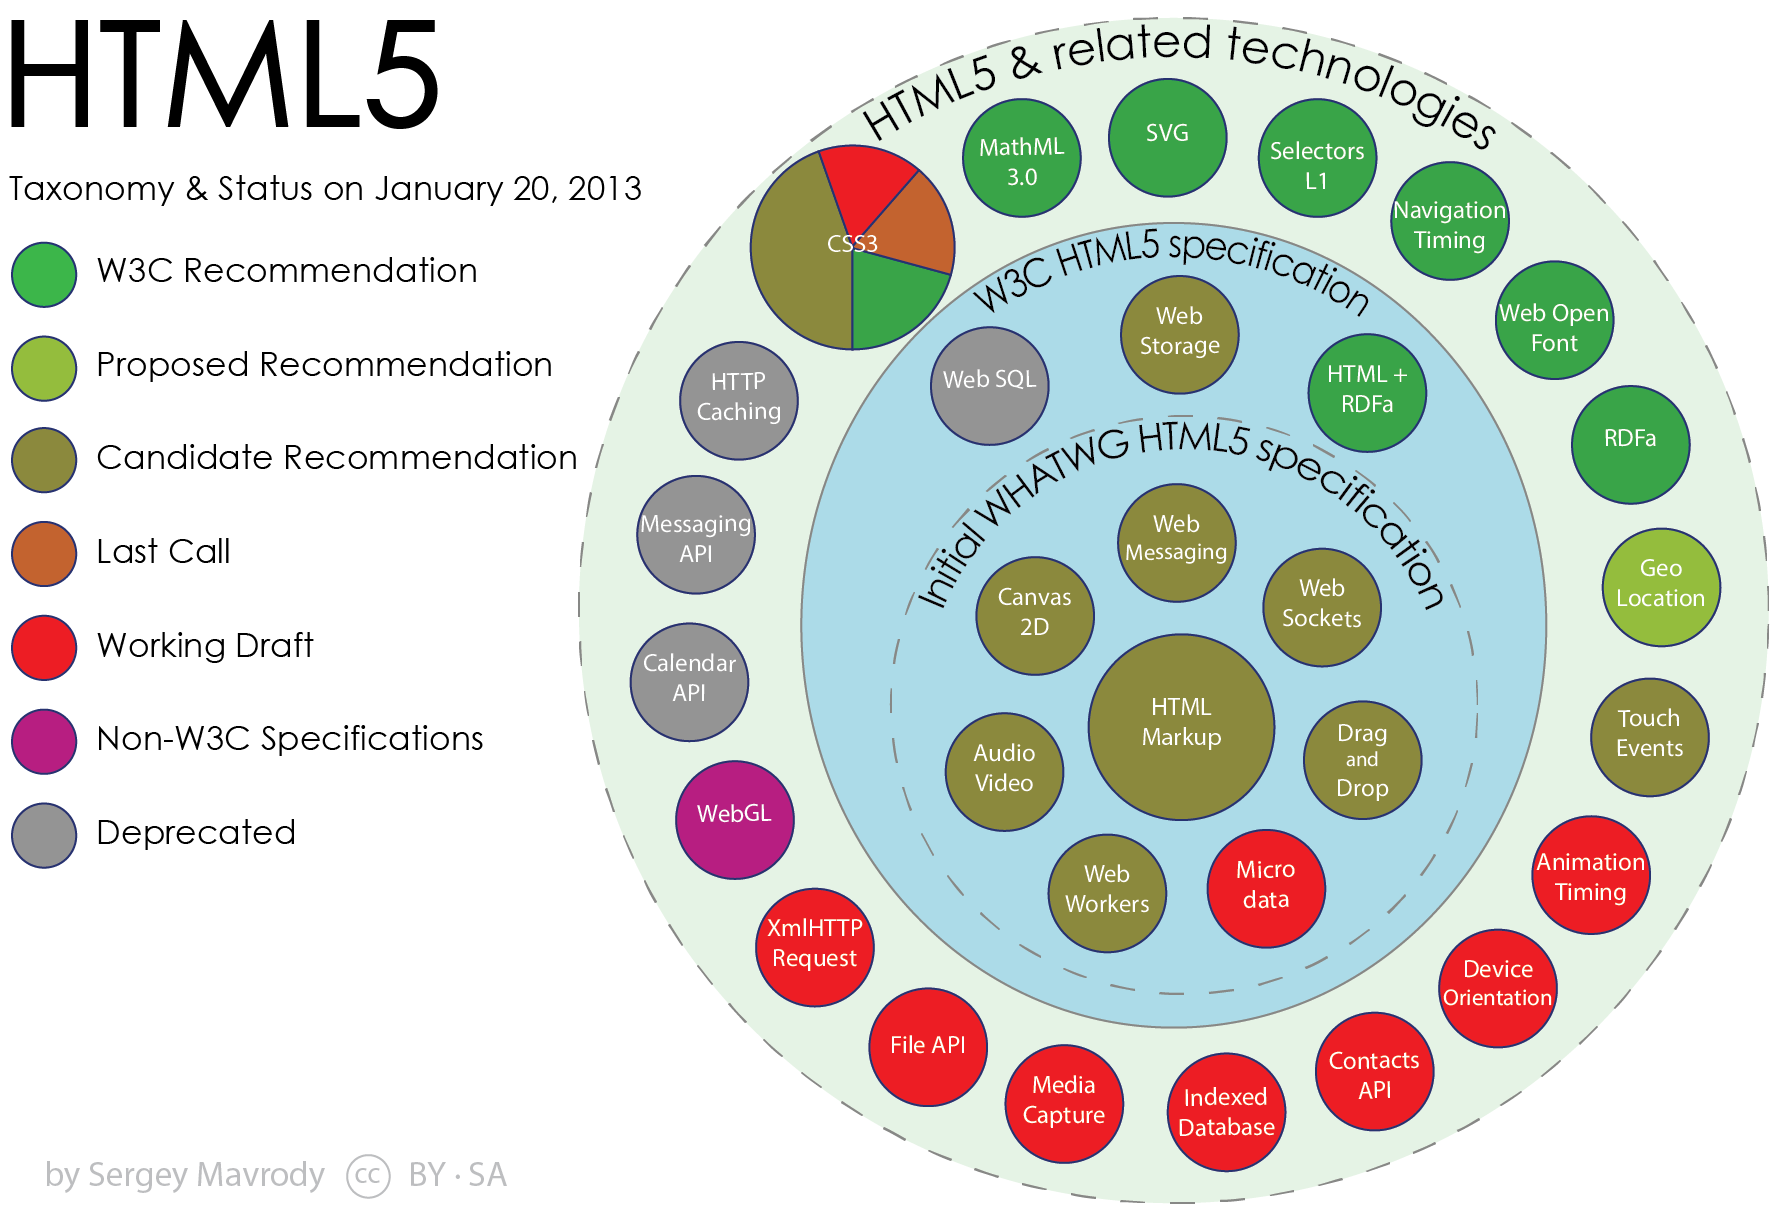
\includegraphics[scale=0.2]{HTML5-APIs-and-related-technologies.png}
\caption{HTML5 APIs and related technologies}
\label{HTML5-APIs-and-related-technologies}
\end{figure}

\chapter{Features}




\section{Markup}


HTML5 introduces elements and attributes that reflect typical usage on modern websites. Some of them are semantic replacements for common uses of generic block (<div>) and inline (<span>) elements, for example <nav> (website navigation block), <footer> (usually referring to bottom of web page or to last lines of HTML code), or <audio> and <video> instead of <object>. Some deprecated elements from HTML 4.01 have been dropped, including purely presentational elements such as <font> and <center>, whose effects have long been superseded by the more capable Cascading Style Sheets. There is also a renewed emphasis on the importance of DOM scripting (e.g., JavaScript) in Web behavior.

The HTML5 syntax is no longer based on SGML despite the similarity of its markup. It has, however, been designed to be backward compatible with common parsing of older versions of HTML. It comes with a new introductory line that looks like an SGML document type declaration, <!DOCTYPE html>, which triggers the standards-compliant rendering mode. As of 5 January 2009, HTML5 also includes Web Forms 2.0, a previously separate WHATWG specification.

通过制定如何处理所有 HTML 元素以及如何从错误中恢复的精确规则,HTML 5 改进了互操作性,并减少了开发成本。

HTML 5 中增加了嵌入音频、视频和图形的功能,客户端数据存储,以及交互式文档。

HTML 5 还包含了新的元素,比如:<nav>, <header>, <footer> 以及 <figure> 等等。


\subsection{HTML 5 Elements}




下面的表格列出了所有的HTML5/HTML 4.01/XHTML 元素,并定义了每个元素可以出现在哪种文档类型声明 (DTD) 中 。


\begin{longtable}{|l|l|l|l|l|l|}
%head
\multicolumn{6}{r}{...}
\tabularnewline\hline
\multirow{2}{80pt}{Tag}	&\multirow{2}{60pt}{HTML5} 	&\multicolumn{3}{c|}{HTML 4.01 / XHTML 1.0}		&\multirow{2}{50pt}{XHTML1.1} \\ \cline{3-5} 
						&							&Transitional		& Strict  	&  Frameset	 		& \multicolumn{1}{c|}{}
\endhead
%endhead

%firsthead
\caption{HTML5/HTML 4.01/XHTML 元素与DTD}\\
\hline
\multirow{2}{60pt}{Tag}	&\multirow{2}{60pt}{HTML5} 	&\multicolumn{3}{c|}{HTML 4.01 / XHTML 1.0}		&\multirow{2}{50pt}{XHTML1.1} \\ \cline{3-5} 
						&							&Transitional		& Strict  	&  Frameset	 		& \multicolumn{1}{c|}{}
\endfirsthead
%endfirsthead

%foot
\multicolumn{6}{r}{...}
\endfoot
%endfoot

\hline

%lastfoot
\endlastfoot
%endlastfoot
\hline
<a>				&Yes	&Yes			&Yes	&Yes				&Yes	\\
\hline
<abbr>			&Yes	&Yes			&Yes	&Yes				&Yes	\\
\hline
<acronym>		&No		&Yes			&Yes	&Yes				&Yes	\\
\hline
<address>		&Yes	&Yes			&Yes	&Yes				&Yes	\\
\hline
<applet>			&No		&Yes			&No		&Yes				&No		\\
\hline
<area>			&Yes	&Yes			&Yes	&Yes				&No		\\
\hline
<article>			&Yes	&No				&No		&No					&No		\\
\hline
<aside>			&Yes	&No				&No		&No					&No		\\
\hline
<audio>			&Yes	&No				&No		&No					&No		\\
\hline
<b>				&Yes	&Yes			&Yes	&Yes				&Yes	\\
\hline
<base>			&Yes	&Yes			&Yes	&Yes				&Yes	\\
\hline
<bdi>			&Yes	&No				&No		&No					&No		\\
\hline
<basefont>		&No		&Yes			&No		&Yes				&No		\\
\hline
<bdo>			&Yes	&Yes			&Yes	&Yes				&No		\\
\hline
<big>			&No		&Yes			&Yes	&Yes				&Yes	\\
\hline
<blockquote>		&Yes	&Yes			&Yes	&Yes				&Yes	\\
\hline
<body>			&Yes	&Yes			&Yes	&Yes				&Yes	\\
\hline
<br>				&Yes	&Yes			&Yes	&Yes				&Yes	\\
\hline
<button>			&Yes	&Yes			&Yes	&Yes				&Yes	\\
\hline
<canvas>			&Yes	&No				&No		&No					&No		\\
\hline
<caption>			&Yes	&Yes			&Yes	&Yes				&Yes	\\
\hline
<center>			&No		&Yes			&No		&Yes				&No		\\
\hline
<cite>			&Yes	&Yes			&Yes	&Yes				&Yes	\\
\hline
<code>			&Yes	&Yes			&Yes	&Yes				&Yes	\\
\hline
<col>			&Yes	&Yes			&Yes	&Yes				&No		\\
\hline
<colgroup>		&Yes	&Yes			&Yes	&Yes				&No		\\
\hline
<command>		&Yes	&No				&No		&No					&No		\\
\hline
<datalist>		&Yes	&No				&No		&No					&No		\\
\hline
<dd>			&Yes	&Yes			&Yes	&Yes				&Yes	\\
\hline
<del>			&Yes	&Yes			&Yes	&Yes				&No		\\
\hline
<details>			&Yes	&No				&No		&No					&No		\\
\hline
<dfn>			&Yes	&Yes			&Yes	&Yes				&Yes	\\
\hline
<dir>			&No		&Yes			&No		&Yes				&No		\\
\hline
<div>			&Yes	&Yes			&Yes	&Yes				&Yes	\\
\hline
<dl>				&Yes	&Yes			&Yes	&Yes				&Yes	\\
\hline
<dt>				&Yes	&Yes			&Yes	&Yes				&Yes	\\
\hline
<em>			&Yes	&Yes			&Yes	&Yes				&Yes	\\
\hline
<embed>			&Yes	&No				&No		&No					&No		\\
\hline
<fieldset>		&Yes	&Yes			&Yes	&Yes				&Yes	\\
\hline
<figcaption>		&Yes	&No				&No		&No					&No		\\
\hline
<figure>			&Yes	&No				&No		&No					&No		\\
\hline
<font>			&No		&Yes			&No		&Yes				&No		\\
\hline
<footer>			&Yes	&No				&No		&No					&No		\\
\hline
<form>			&Yes	&Yes			&Yes	&Yes				&Yes	\\
\hline
<frame>			&No		&No				&No		&Yes				&No		\\
\hline
<frameset>		&No		&No				&No		&Yes				&No		\\
\hline
<h1> to <h6>		&Yes	&Yes			&Yes	&Yes				&Yes	\\
\hline
<head>			&Yes	&Yes			&Yes	&Yes				&Yes	\\
\hline
<header>			&Yes	&No				&No		&No					&No		\\
\hline
<hgroup>			&Yes	&No				&No		&No					&No		\\
\hline
<hr>				&Yes	&Yes			&Yes	&Yes				&Yes	\\
\hline
<html>			&Yes	&Yes			&Yes	&Yes				&Yes	\\
\hline
<i>				&Yes	&Yes			&Yes	&Yes				&Yes	\\
\hline
<iframe>			&Yes	&Yes			&No		&Yes				&No		\\
\hline
<img>			&Yes	&Yes			&Yes	&Yes				&Yes	\\
\hline
<input>			&Yes	&Yes			&Yes	&Yes				&Yes	\\
\hline
<ins>			&Yes	&Yes			&Yes	&Yes				&No		\\
\hline
<isindex>			&No		&Yes			&No		&Yes				&No		\\
\hline
<kbd>			&Yes	&Yes			&Yes	&Yes				&Yes	\\
\hline
<keygen>			&Yes	&No				&No		&No					&No		\\
\hline
<label>			&Yes	&Yes			&Yes	&Yes				&Yes	\\
\hline
<legend>			&Yes	&Yes			&Yes	&Yes				&Yes	\\
\hline
<li>				&Yes	&Yes			&Yes	&Yes				&Yes	\\
\hline
<link>			&Yes	&Yes			&Yes	&Yes				&Yes	\\
\hline
<map>			&Yes	&Yes			&Yes	&Yes				&No		\\
\hline
<menu>			&Yes	&Yes			&No		&Yes				&No		\\
\hline
<meta>			&Yes	&Yes			&Yes	&Yes				&Yes	\\
\hline
<meter>			&Yes	&No				&No		&No					&No		\\
\hline
<nav>			&Yes	&No				&No		&No					&No		\\
\hline
<noframes>		&No		&Yes			&No		&Yes				&No		\\
\hline
<noscript>		&Yes	&Yes			&Yes	&Yes				&Yes	\\
\hline
<object>			&Yes	&Yes			&Yes	&Yes				&Yes	\\
\hline
<ol>				&Yes	&Yes			&Yes	&Yes				&Yes	\\
\hline
<optgroup>		&Yes	&Yes			&Yes	&Yes				&Yes	\\
\hline
<option>			&Yes	&Yes			&Yes	&Yes				&Yes	\\
\hline
<output>			&Yes	&No				&No		&No					&No		\\
\hline
<p>				&Yes	&Yes			&Yes	&Yes				&Yes	\\
\hline
<param>			&Yes	&Yes			&Yes	&Yes				&Yes	\\
\hline
<pre>			&Yes	&Yes			&Yes	&Yes				&Yes	\\
\hline
<progress>		&Yes	&No				&No		&No					&No		\\
\hline
<q>				&Yes	&Yes			&Yes	&Yes				&Yes	\\
\hline
<rp>				&Yes	&No				&No		&No					&No		\\
\hline
<rt>				&Yes	&No				&No		&No					&No		\\
\hline
<ruby>			&Yes	&No				&No		&No					&No		\\
\hline
<s>				&Yes	&Yes			&No		&Yes				&No		\\
\hline
<samp>			&Yes	&Yes			&Yes	&Yes				&Yes	\\
\hline
<script>			&Yes	&Yes			&Yes	&Yes				&Yes	\\
\hline
<section>			&Yes	&No				&No		&No					&No		\\
\hline
<select>			&Yes	&Yes			&Yes	&Yes				&Yes	\\
\hline
<small>			&Yes	&Yes			&Yes	&Yes				&Yes	\\
\hline
<source>			&Yes	&No				&No		&No					&No		\\
\hline
<span>			&Yes	&Yes			&Yes	&Yes				&Yes	\\
\hline
<strike>			&No		&Yes			&No		&Yes				&No		\\
\hline
<strong>			&Yes	&Yes			&Yes	&Yes				&Yes	\\
\hline
<style>			&Yes	&Yes			&Yes	&Yes				&Yes	\\
\hline
<sub>			&Yes	&Yes			&Yes	&Yes				&Yes	\\
\hline
<summary>		&Yes	&No				&No		&No					&No		\\
\hline
<sup>			&Yes	&Yes			&Yes	&Yes				&Yes	\\
\hline
<table>			&Yes	&Yes			&Yes	&Yes				&Yes	\\
\hline
<tbody>			&Yes	&Yes			&Yes	&Yes				&No		\\
\hline
<td>				&Yes	&Yes			&Yes	&Yes				&Yes	\\
\hline
<textarea>		&Yes	&Yes			&Yes	&Yes				&Yes	\\
\hline
<tfoot>			&Yes	&Yes			&Yes	&Yes				&No		\\
\hline
<th>				&Yes	&Yes			&Yes	&Yes				&Yes	\\
\hline
<thead>			&Yes	&Yes			&Yes	&Yes				&No		\\
\hline
<time>			&Yes	&No				&No		&No					&No		\\
\hline
<title>			&Yes	&Yes			&Yes	&Yes				&Yes	\\
\hline
<tr>				&Yes	&Yes			&Yes	&Yes				&Yes	\\
\hline
<track>			&Yes	&No				&No		&No					&No		\\
\hline
<tt>				&No		&Yes			&Yes	&Yes				&Yes	\\
\hline
<u>				&No		&Yes			&No		&Yes				&No		\\
\hline
<ul>				&Yes	&Yes			&Yes	&Yes				&Yes	\\
\hline
<var>			&Yes	&Yes			&Yes	&Yes				&Yes	\\
\hline
<video>			&Yes	&No				&No		&No					&No		\\
\hline
<wbr>			&Yes	&No				&No		&No					&No		\\
\hline
\end{longtable}



\subsection{HTML 5 Attributes}

所有 HTML 5 标签均支持下面列出的属性\footnote{注释:HTML 4.01 不再支持 accesskey 属性:},仅有少数例外。

\begin{longtable}{|p{70pt}|p{70pt}|p{230pt}|}
%head
\multicolumn{3}{r}{}
\tabularnewline\hline
属性	&值	&描述
\endhead
%endhead

%firsthead
\caption{HTML 5 Attributes}\\
\hline
属性	&值	&描述
\endfirsthead
%endfirsthead

%foot
\multicolumn{3}{r}{}
\endfoot
%endfoot

%lastfoot
\endlastfoot
%endlastfoot
\hline
accesskey	&character			&规定访问元素的键盘快捷键\\
\hline
class		&classname			&规定元素的类名(用于规定样式表中的类)。\\
\hline
contenteditable&true \newline false	&规定是否允许用户编辑内容。\\
\hline
contextmenu	&menu\_id			&规定元素的上下文菜单。\\
\hline
data-yourvalue&value				&创作者定义的属性。\newline HTML 文档的创作者可以定义他们自己的属性。\newline 必须以``data-" 开头。\\
\hline
dir			& ltr \newline rtl		&规定元素中内容的文本方向。\\
\hline
draggable	& true\newline false \newline auto &规定是否允许用户拖动元素。\\
\hline
hidden		&hidden				&规定该元素是无关的。被隐藏的元素不会显示。\\
\hline
id			&id					&规定元素的唯一 ID。\\
\hline
item			&empty \newline url 	&用于组合元素。\\
\hline
itemprop		&url \newline group value&用于组合项目。\\
\hline
lang			&language\_code		&规定元素中内容的语言代码。\\
\hline
spellcheck	&true\newline false	&规定是否必须对元素进行拼写或语法检查。\\
\hline
style		&style\_definition		&规定元素的行内样式。\\
\hline
subject		&id					&规定元素对应的项目。\\
\hline
tabindex		&number				&规定元素的 tab 键控制次序。\\
\hline
title			&text				&规定有关元素的额外信息。\\
\hline

\end{longtable}


\subsection{HTML 5 Events}

HTML 4 增加了通过事件触发浏览器中行为的能力,比如当用户点击某个元素时启动一段 JavaScript。

下面的表格列出了可插入 HTML 5 元素中以定义事件行为的标准事件属性。


\begin{compactitem}
\item Window 事件属性 - Window Event Attributes
\item 表单事件 - Form Events
\item 键盘事件 - Keybord Events
\item 鼠标事件 - Mouse Events
\item 媒介事件 - Media Events
\end{compactitem}


\subsubsection{HTML 5 Window Event Attributes}

window 对象触发的事件,适用于 <body> 标签。

\CTEXnoindent
\begin{longtable}{|p{90pt}|p{40pt}|p{240pt}|}
%head
\multicolumn{3}{r}{}
\tabularnewline\hline
属性	&值	&描述
\endhead
%endhead

%firsthead
\caption{HTML 5 Window Event Attributes}\\
\hline
属性	&值	&描述
\endfirsthead
%endfirsthead

%foot
\multicolumn{3}{r}{}
\endfoot
%endfoot

%lastfoot
\endlastfoot
%endlastfoot
\hline

onafterprint		&script	&在打印文档之后运行脚本\\
\hline
onbeforeprint		&script	&在文档打印之前运行脚本\\
\hline
onbeforeonload	&script	&在文档加载之前运行脚本\\
\hline
onblur			&script	&当窗口失去焦点时运行脚本\\
\hline
onerror			&script	&当错误发生时运行脚本\\
\hline
onfocus			&script	&当窗口获得焦点时运行脚本\\
\hline
onhaschange		&script	&当文档改变时运行脚本\\
\hline
onload			&script	&当文档加载时运行脚本\\
\hline
onmessage		&script	&当触发消息时运行脚本\\
\hline
onoffline			&script	&当文档离线时运行脚本\\
\hline
ononline			&script	&当文档上线时运行脚本\\
\hline
onpagehide		&script	&当窗口隐藏时运行脚本\\
\hline
onpageshow		&script	&当窗口可见时运行脚本\\
\hline
onpopstate		&script	&当窗口历史记录改变时运行脚本\\
\hline
onredo			&script	&当文档执行再执行操作(redo)时运行脚本\\
\hline
onresize			&script	&当调整窗口大小时运行脚本\\
\hline
onstorage		&script	&当文档加载加载时运行脚本\\
\hline
onundo			&script	&当 Web Storage 区域更新时(存储空间中的数据发生变化时)\\
\hline
onunload			&script	&当用户离开文档时运行脚本\\
\hline
\end{longtable}


\CTEXindent


\subsubsection{HTML 5 Form Events}


由 HTML 表单内部的动作触发的事件,适用于所有 HTML 5 元素,不过最常用于表单元素中。

\begin{longtable}{|p{90pt}|p{40pt}|p{240pt}|}
%head
\multicolumn{3}{r}{}
\tabularnewline\hline
属性	&值	&描述
\endhead
%endhead

%firsthead
\caption{HTML 5 Form Events}\\
\hline
属性	&值	&描述
\endfirsthead
%endfirsthead

%foot
\multicolumn{3}{r}{}
\endfoot
%endfoot

%lastfoot
\endlastfoot
%endlastfoot
\hline
onblur			&script	&当元素失去焦点时运行脚本\\
\hline
onchange			&script	&当元素改变时运行脚本\\
\hline
oncontextmenu	&script	&当触发上下文菜单时运行脚本\\
\hline
onfocus			&script	&当元素获得焦点时运行脚本\\
\hline
onformchange		&script	&当表单改变时运行脚本\\
\hline
onforminput		&script	&当表单获得用户输入时运行脚本\\
\hline
oninput			&script	&当元素获得用户输入时运行脚本\\
\hline
oninvalid			&script	&当元素无效时运行脚本\\
\hline
onreset			&script	&当表单重置时运行脚本。HTML 5 不支持。\\
\hline
onselect			&script	&当选取元素时运行脚本\\
\hline
onsubmit			&script	&当提交表单时运行脚本\\
\hline
\end{longtable}


\subsubsection{HTML 5 Keyboard Events}

由键盘触发的事件,适用于所有 HTML 5 元素。

\begin{longtable}{|p{90pt}|p{40pt}|p{240pt}|}
%head
\multicolumn{3}{r}{}
\tabularnewline\hline
属性	&值	&描述
\endhead
%endhead

%firsthead
\caption{HTML 5 Keyboard Events}\\
\hline
属性	&值	&描述
\endfirsthead
%endfirsthead

%foot
\multicolumn{3}{r}{}
\endfoot
%endfoot

%lastfoot
\endlastfoot
%endlastfoot
\hline
onkeydown	&script	&当按下按键时运行脚本\\
\hline
onkeypress	&script	&当按下并松开按键时运行脚本\\
\hline
onkeyup		&script	&当松开按键时运行脚本\\
\hline

\end{longtable}


\subsubsection{HTML 5 Mouse Events}

由鼠标或相似的用户动作触发的事件,适用于所有 HTML 5 元素。

\begin{longtable}{|p{90pt}|p{40pt}|p{240pt}|}
%head
\multicolumn{3}{r}{}
\tabularnewline\hline
属性	&值	&描述
\endhead
%endhead

%firsthead
\caption{HTML 5 Mouse Events}\\
\hline
属性	&值	&描述
\endfirsthead
%endfirsthead

%foot
\multicolumn{3}{r}{}
\endfoot
%endfoot

%lastfoot
\endlastfoot
%endlastfoot
\hline
onclick		&script	&当单击鼠标时运行脚本\\
\hline
ondblclick	&script	&当双击鼠标时运行脚本\\
\hline
ondrag		&script	&当拖动元素时运行脚本\\
\hline
ondragend	&script	&当拖动操作结束时运行脚本\\
\hline
ondragenter	&script	&当元素被拖动至有效的拖放目标时运行脚本\\
\hline
ondragleave	&script	&当元素离开有效拖放目标时运行脚本\\
\hline
ondragover	&script	&当元素被拖动至有效拖放目标上方时运行脚本\\
\hline
ondragstart	&script	&当拖动操作开始时运行脚本\\
\hline
ondrop		&script	&当被拖动元素正在被拖放时运行脚本\\
\hline
onmousedown	&script	&当按下鼠标按钮时运行脚本\\
\hline
onmousemove	&script	&当鼠标指针移动时运行脚本\\
\hline
onmouseout	&script	&当鼠标指针移出元素时运行脚本\\
\hline
onmouseover	&script	&当鼠标指针移至元素之上时运行脚本\\
\hline
onmouseup	&script	&当松开鼠标按钮时运行脚本\\
\hline
onmousewheel&script	&当转动鼠标滚轮时运行脚本\\
\hline
onscroll		&script	&当滚动元素滚动元素的滚动条时运行脚本\\
\hline
\end{longtable}

\subsubsection{HTML 5 Media Events}

由视频、图像以及音频等媒介触发的事件,适用于所有 HTML 5 元素,不过在媒介元素(诸如 audio、embed、img、object 以及 video)中最常用。


\begin{longtable}{|p{90pt}|p{40pt}|p{240pt}|}
%head
\multicolumn{3}{r}{}
\tabularnewline\hline
属性	&值	&描述
\endhead
%endhead

%firsthead
\caption{HTML 5 Media Events}\\
\hline
属性	&值	&描述
\endfirsthead
%endfirsthead

%foot
\multicolumn{3}{r}{}
\endfoot
%endfoot

%lastfoot
\endlastfoot
%endlastfoot
\hline
onabort			&script	&当发生中止事件时运行脚本\\
\hline
oncanplay		&script	&当媒介能够开始播放但可能因缓冲而需要停止时运行脚本\\
\hline
oncanplaythrough	&script	&当媒介能够无需因缓冲而停止即可播放至结尾时运行脚本\\
\hline
ondurationchange	&script	&当媒介长度改变时运行脚本\\
\hline
onemptied		&script	&当媒介资源元素突然为空时(网络错误、加载错误等)运行脚本\\
\hline
onended			&script	&当媒介已抵达结尾时运行脚本\\
\hline
onerror			&script	&当在元素加载期间发生错误时运行脚本\\
\hline
onloadeddata		&script	&当加载媒介数据时运行脚本\\
\hline
onloadedmetadata	&script	&当媒介元素的持续时间以及其他媒介数据已加载时运行脚本\\
\hline
onloadstart		&script	&当浏览器开始加载媒介数据时运行脚本\\
\hline
onpause			&script	&当媒介数据暂停时运行脚本\\
\hline
onplay			&script	&当媒介数据将要开始播放时运行脚本\\
\hline
onplaying			&script	&当媒介数据已开始播放时运行脚本\\
\hline
onprogress		&script	&当浏览器正在取媒介数据时运行脚本\\
\hline
onratechange		&script	&当媒介数据的播放速率改变时运行脚本\\
\hline
onreadystatechange&script	&当就绪状态(ready-state)改变时运行脚本\\
\hline
onseeked			&script	&当媒介元素的定位属性(seeking attribute)不再为真且定位已结束时运行脚本\\
\hline
onseeking		&script	&当媒介元素的定位属性为真且定位已开始时运行脚本\\
\hline
onstalled			&script	&当取回媒介数据过程中(延迟)存在错误时运行脚本\\
\hline
onsuspend		&script	&当浏览器已在取媒介数据但在取回整个媒介文件之前停止时运行脚本\\
\hline
ontimeupdate		&script	&当媒介改变其播放位置时运行脚本\\
\hline
onvolumechange	&script	&当媒介改变音量亦或当音量被设置为静音时运行脚本\\
\hline
onwaiting			&script	&当媒介已停止播放但打算继续播放时运行脚本\\
\hline
\end{longtable}


\section{HTML 5 Input}

HTML5 拥有多个新的表单输入类型,这些新特性提供了更好的输入控制和验证。


\begin{compactitem}
\item email
\item url
\item number
\item range
\item Date pickers (date, month, week, time, datetime, datetime-local)
\item search
\item color
\end{compactitem}

\begin{longtable}{|p{80pt}|p{50pt}|p{50pt}|p{50pt}|p{50pt}|p{50pt}|}
%head
\multicolumn{6}{r}{}
\tabularnewline\hline
Input type	&IE	&Firefox	&Opera	&Chrome	&Safari
\endhead
%endhead

%firsthead
\caption{HTML 5 Input 类型}\\
\hline
Input type	&IE	&Firefox	&Opera	&Chrome	&Safari
\endfirsthead
%endfirsthead

%foot
\multicolumn{6}{r}{}
\endfoot
%endfoot

%lastfoot
\endlastfoot
%endlastfoot
\hline
email	&No		&4.0	&9.0	&10.0	&No\\
\hline
url		&No		&4.0	&9.0	&10.0	&No\\
\hline
number	&No		&No		&9.0	&7.0	&No\\
\hline
range	&No		&No		&9.0	&4.0	&4.0\\
\hline
Date pickers&	No	&No		&9.0	&10.0	&No\\
\hline
search	&No		&4.0	&11.0	&10.0	&No\\
\hline
color	&No		&No		&11.0	&No		&No\\
\hline
\end{longtable}



Opera 对新的输入类型的支持最好。不过即使在其他浏览器中不被支持,仍然可以显示为常规的文本域。

\subsection{email}

email 类型用于应该包含 e-mail 地址的输入域。在提交表单时,会自动验证 email 域的值。

\begin{lstlisting}[language=HTML]
E-mail: <input type="email" name="user_email" />
\end{lstlisting}

iPhone 中的 Safari 浏览器支持 email 输入类型,并通过改变触摸屏键盘来配合它(添加 @ 和 .com 选项)。


\subsection{url}

url 类型用于应该包含 URL 地址的输入域。在提交表单时,会自动验证 url 域的值。

\begin{lstlisting}[language=HTML]
Homepage: <input type="url" name="user_url" />
\end{lstlisting}

iPhone 中的 Safari 浏览器支持 url 输入类型,并通过改变触摸屏键盘来配合它(添加 .com 选项)。


\subsection{number}

number 类型用于应该包含数值的输入域。另外,还可以设定对所接受的数字的限定:

\begin{lstlisting}[language=HTML]
Points: <input type="number" name="points" min="1" max="10" />
\end{lstlisting}

使用下面的属性来规定对数字类型的限定:

\begin{longtable}{|p{80pt}|p{50pt}|p{200pt}|}
%head
\multicolumn{3}{r}{}
\tabularnewline\hline
属性	&值	&描述
\endhead
%endhead

%firsthead
\caption{HTML 5 数字类型的限定}\\
\hline
属性	&值	&描述
\endfirsthead
%endfirsthead

%foot
\multicolumn{3}{r}{}
\endfoot
%endfoot

%lastfoot
\endlastfoot
%endlastfoot
\hline
max	&number	&规定允许的最大值\\
\hline
min	&number	&规定允许的最小值\\
\hline
step	&number	&规定合法的数字间隔(如果 step="3",则合法的数是 -3,0,3,6 等)\\
\hline
value&number	&规定默认值\\
\hline

\end{longtable}

iPhone 中的 Safari 浏览器支持 number 输入类型,并通过改变触摸屏键盘来配合它(显示数字)。



\subsection{range}

range 类型用于应该包含一定范围内数字值的输入域。range 类型显示为滑动条。

另外,也能够设定对所接受的数字的限定:

\begin{lstlisting}[language=HTML]
<input type="range" name="points" min="1" max="10" />
\end{lstlisting}

使用下面的属性来规定对数字类型的限定:


\begin{longtable}{|p{80pt}|p{50pt}|p{200pt}|}
%head
\multicolumn{3}{r}{}
\tabularnewline\hline
属性	&值	&描述
\endhead
%endhead

%firsthead
\caption{HTML 5 数字类型的限定}\\
\hline
属性	&值	&描述
\endfirsthead
%endfirsthead

%foot
\multicolumn{3}{r}{}
\endfoot
%endfoot

%lastfoot
\endlastfoot
%endlastfoot
\hline
max	&number	&规定允许的最大值\\
\hline
min	&number	&规定允许的最小值\\
\hline
step	&number	&规定合法的数字间隔(如果 step="3",则合法的数是 -3,0,3,6 等)\\
\hline
value&number	&规定默认值\\
\hline

\end{longtable}





\subsection{Date Pickers}


HTML5 拥有多个可供选取日期和时间的新输入类型:


\begin{compactitem}
\item date - 选取日、月、年
\item month - 选取月、年
\item week - 选取周和年
\item time - 选取时间(小时和分钟)
\item datetime - 选取时间、日、月、年(UTC 时间)
\item datetime-local - 选取时间、日、月、年(本地时间)
\end{compactitem}

下面的例子允许用户从日历中选取一个日期:

\begin{lstlisting}[language=HTML]
Date: <input type="date" name="user_date" />
\end{lstlisting}

\subsection{search}


search 类型用于搜索域,比如站点搜索或 Google 搜索。search 域显示为常规的文本域。




\section{HTML 5 Form}


HTML 5新的表单元素包括:

\begin{compactitem}
\item datalist
\item keygen
\item output
\end{compactitem}



HTML5 拥有若干涉及表单的元素和属性。


\begin{longtable}{|p{80pt}|p{50pt}|p{50pt}|p{50pt}|p{50pt}|p{50pt}|}
%head
\multicolumn{6}{r}{}
\tabularnewline\hline
Input type	&IE	&Firefox	&Opera	&Chrome	&Safari
\endhead
%endhead

%firsthead
\caption{HTML 5 Form 类型}\\
\hline
Input type	&IE	&Firefox	&Opera	&Chrome	&Safari
\endfirsthead
%endfirsthead

%foot
\multicolumn{6}{r}{}
\endfoot
%endfoot

%lastfoot
\endlastfoot
%endlastfoot
\hline
datalist	&No		&No		&9.5	&No		&No\\
\hline
keygen	&No		&No		&10.5	&3.0	&No\\
\hline
output	&No		&No		&9.5	&No		&No\\
\hline

\end{longtable}



\subsection{datalist}


datalist 元素规定输入域的选项列表。

列表是通过 datalist 内的 option 元素\footnote{提示:option 元素永远都要设置 value 属性。}创建的。

如需把 datalist 绑定到输入域,需要用输入域的 list 属性引用 datalist 的 id:

\begin{lstlisting}[language=HTML]
Webpage: <input type="url" list="url_list" name="link" />
<datalist id="url_list">
<option label="W3School" value="http://www.W3School.com.cn" />
<option label="Google" value="http://www.google.com" />
<option label="Microsoft" value="http://www.microsoft.com" />
</datalist>
\end{lstlisting}






\subsection{keygen}

keygen 元素的作用是提供一种验证用户的可靠方法\footnote{目前,浏览器对此元素的糟糕的支持度不足以使其成为一种有用的安全标准。}。

keygen 元素是密钥对生成器(key-pair generator)。当提交表单时,会生成两个键,一个是私钥,一个公钥。

私钥(private key)存储于客户端,公钥(public key)则被发送到服务器。公钥可用于之后验证用户的客户端证书(client certificate)。

\begin{lstlisting}[language=HTML]
<form action="demo_form.asp" method="get">
Username: <input type="text" name="usr_name" />
Encryption: <keygen name="security" />
<input type="submit" />
</form>
\end{lstlisting}


\subsection{output}


output 元素用于不同类型的输出,比如计算或脚本输出:

\begin{lstlisting}[language=HTML]
<output id="result" onforminput="resCalc()"></output>
\end{lstlisting}


\begin{longtable}{|p{80pt}|p{50pt}|p{50pt}|p{50pt}|p{50pt}|p{50pt}|}
%head
\multicolumn{6}{r}{}
\tabularnewline\hline
Input type	&IE	&Firefox	&Opera	&Chrome	&Safari
\endhead
%endhead

%firsthead
\caption{HTML 5 表单属性}\\
\hline
Input type	&IE	&Firefox	&Opera	&Chrome	&Safari
\endfirsthead
%endfirsthead

%foot
\multicolumn{6}{r}{}
\endfoot
%endfoot

%lastfoot
\endlastfoot
%endlastfoot
\hline
autocomplete	&8.0	&3.5	&9.5	&3.0	&4.0\\
\hline
autofocus	&No		&No		&10.0	&3.0	&4.0\\
\hline
form			&No		&No		&9.5	&No		&No\\
\hline
form overrides	&No		&No		&10.5	&No		&No\\
\hline
height and width&	8.0	&3.5	&9.5	&3.0	&4.0\\
\hline
list			&No		&No		&9.5	&No		&No\\
\hline
min, max and step&	No	&No		&9.5	&3.0	&No\\
\hline
multiple		&No		&3.5	&No		&3.0	&4.0\\
\hline
novalidate	&No		&No		&No		&No		&No\\
\hline
pattern		&No		&No		&9.5	&3.0	&No\\
\hline
placeholder	&No		&No		&No		&3.0	&3.0\\
\hline
required		&No		&No		&9.5	&3.0	&No\\
\hline

\end{longtable}



\subsection{autocomplete}

autocomplete\footnote{注释:autocomplete 适用于 <form> 标签,以及以下类型的 <input> 标签:text, search, url, telephone, email, password, datepickers, range 以及 color。} 属性规定 form 或 input 域应该拥有自动完成功能。

当用户在自动完成域中开始输入时,浏览器应该在该域中显示填写的选项:

\begin{lstlisting}[language=HTML]
<form action="demo_form.asp" method="get" autocomplete="on">
First name: <input type="text" name="fname" /><br />
Last name: <input type="text" name="lname" /><br />
E-mail: <input type="email" name="email" autocomplete="off" /><br />
<input type="submit" />
</form>
\end{lstlisting}

注释:在某些浏览器中,可能需要启用自动完成功能,以使该属性生效。


\subsection{autofocus}


autofocus\footnote{注释:autofocus 属性适用于所有 <input> 标签的类型。} 属性规定在页面加载时,域自动地获得焦点。

\begin{lstlisting}[language=HTML]
User name: <input type="text" name="user_name"  autofocus="autofocus" />
\end{lstlisting}



\subsection{form}

form\footnote{注释:form 属性适用于所有 <input> 标签的类型。} 属性规定输入域所属的一个或多个表单。

form 属性必须引用所属表单的 id:


\begin{lstlisting}[language=HTML]
<form action="demo_form.asp" method="get" id="user_form">
First name:<input type="text" name="fname" />
<input type="submit" />
</form>
Last name: <input type="text" name="lname" form="user_form" />
\end{lstlisting}

注释:如需引用一个以上的表单,需要使用空格分隔的列表。

\subsection{override}

表单重写属性(form override attributes)\footnote{注释:表单重写属性适用于以下类型的 <input> 标签:submit 和 image。}允许开发者重写 form 元素的某些属性设定。


表单重写属性有:

\begin{compactitem}
\item formaction - 重写表单的 action 属性
\item formenctype - 重写表单的 enctype 属性
\item formmethod - 重写表单的 method 属性
\item formnovalidate - 重写表单的 novalidate 属性
\item formtarget - 重写表单的 target 属性
\end{compactitem}


\begin{lstlisting}[language=HTML]
<form action="demo_form.asp" method="get" id="user_form">
E-mail: <input type="email" name="userid" /><br />
<input type="submit" value="Submit" />
<br />
<input type="submit" formaction="demo_admin.asp" value="Submit as admin" />
<br />
<input type="submit" formnovalidate="true" value="Submit without validation" />
<br />
</form>
\end{lstlisting}

注释:这些属性对于创建不同的提交按钮很有帮助。


\subsection{height \& width}

height\footnote{注释:height 和 width 属性只适用于 image 类型的 <input> 标签。} 和 width\footnote{注释:height 和 width 属性只适用于 image 类型的 <input> 标签。} 属性规定用于 image 类型的 input 标签的图像高度和宽度。

\begin{lstlisting}[language=HTML]
<input type="image" src="img_submit.gif" width="99" height="99" />
\end{lstlisting}




\subsection{list}

list\footnote{注释:list 属性适用于以下类型的 <input> 标签:text, search, url, telephone, email, date pickers, number, range 以及 color。} 属性规定输入域的 datalist,datalist 是输入域的选项列表。


\begin{lstlisting}[language=HTML]
Webpage: <input type="url" list="url_list" name="link" />
<datalist id="url_list">
<option label="W3Schools" value="http://www.w3school.com.cn" />
<option label="Google" value="http://www.google.com" />
<option label="Microsoft" value="http://www.microsoft.com" />
</datalist>
\end{lstlisting}



\subsection{min, max, step}

min\footnote{注释:min、max 和 step 属性适用于以下类型的 <input> 标签:date pickers、number 以及 range。}、max\footnote{注释:min、max 和 step 属性适用于以下类型的 <input> 标签:date pickers、number 以及 range。} 和 step\footnote{注释:min、max 和 step 属性适用于以下类型的 <input> 标签:date pickers、number 以及 range。} 属性用于为包含数字或日期的 input 类型规定限定(约束),其中:

\begin{compactitem}
\item max 属性规定输入域所允许的最大值。
\item min 属性规定输入域所允许的最小值。
\item step 属性为输入域规定合法的数字间隔(如果 step="3",则合法的数是 -3,0,3,6 等)。
\end{compactitem}

下面的例子显示一个数字域,该域接受介于 0 到 10 之间的值,且步进为 3(即合法的值为 0、3、6 和 9):

\begin{lstlisting}[language=HTML]
Points: <input type="number" name="points" min="0" max="10" step="3" />
\end{lstlisting}


\subsection{multiple}

multiple\footnote{注释:multiple 属性适用于以下类型的 <input> 标签:email 和 file。} 属性规定输入域中可选择多个值。


\begin{lstlisting}[language=HTML]
Select images: <input type="file" name="img" multiple="multiple" />
\end{lstlisting}



\subsection{novalidate}


novalidate\footnote{注释:novalidate 属性适用于 <form> 以及以下类型的 <input> 标签:text, search, url, telephone, email, password, date pickers, range 以及 color.} 属性规定在提交表单时不应该验证 form 或 input 域。

\begin{lstlisting}[language=HTML]
<form action="demo_form.asp" method="get" novalidate="true">
E-mail: <input type="email" name="user_email" />
<input type="submit" />
</form>
\end{lstlisting}


\subsection{pattern}

pattern\footnote{注释:pattern 属性适用于以下类型的 <input> 标签:text, search, url, telephone, email 以及 password。} 属性规定用于验证 input 域的模式(pattern),模式(pattern) 是正则表达式。


下面的例子显示了一个只能包含三个字母的文本域(不含数字及特殊字符):

\begin{lstlisting}[language=HTML]
Country code: <input type="text" name="country_code"
pattern="[A-z]{3}" title="Three letter country code" />
\end{lstlisting}



\subsection{placeholder}

placeholder\footnote{注释:placeholder 属性适用于以下类型的 <input> 标签:text, search, url, telephone, email 以及 password。} 属性提供一种提示(hint),描述输入域所期待的值。

提示(hint)会在输入域为空时显示出现,会在输入域获得焦点时消失:

\begin{lstlisting}[language=HTML]
<input type="search" name="user_search"  placeholder="Search" />
\end{lstlisting}


\subsection{required}

required\footnote{注释:required 属性适用于以下类型的 <input> 标签:text, search, url, telephone, email, password, date pickers, number, checkbox, radio 以及 file。} 属性规定必须在提交之前填写输入域(不能为空)。


\begin{lstlisting}[language=HTML]
Name: <input type="text" name="usr_name" required="required" />
\end{lstlisting}




\section{APIs}


In addition to specifying markup, HTML5 specifies scripting application programming interfaces (APIs) that can be used with JavaScript. Existing document object model (DOM) interfaces are extended and de facto features documented. There are also new APIs, such as:

\begin{compactitem}
\item The canvas element for immediate mode 2D drawing. 
\item Timed media playback
\item Offline Web Applications
\item Document editing
\item Drag-and-drop
\item Cross-document messaging
\item Browser history management
\item MIME type and protocol handler registration
\item Microdata
\item Web Storage, a key-value pair storage framework that provides behaviour similar to cookies but with larger storage capacity and improved API
\end{compactitem}


Not all of the above technologies are included in the W3C HTML5 specification, though they are in the WHATWG HTML specification. Some related technologies, which are not part of either the W3C HTML5 or the WHATWG HTML specification, are as follows. The W3C publishes specifications for these separately:

\begin{compactitem}
\item Geolocation
\item Web SQL Database, a local SQL Database (no longer maintained).
\item The Indexed Database API, an indexed hierarchical key-value store (formerly WebSimpleDB).
\item HTML5 File API, handles file uploads and file manipulation.
\item Directories and System, an API intended to satisfy client-side-storage use cases not well served by databases.
\item File Writer, an API for writing to files from web applications.
\item Web Audio API, a high-level JavaScript API for processing and synthesizing audio in web applications.
\end{compactitem}

HTML5 alone cannot provide animation within web pages. Either JavaScript or CSS3 is necessary for animating HTML elements. Animation is also possible using JavaScript and HTML 4, and within SVG elements through SMIL, although browser support of the latter remains uneven as of 2011.

\section{2D drawing}

HTML5 的 canvas 元素使用 JavaScript 在网页上绘制图像,canvas 拥有多种绘制路径、矩形、圆形、字符以及添加图像的方法。

画布是一个矩形区域,开发者可以控制其每一像素。不过,<canvas> 元素本身并没有绘制能力(它仅仅是图形的容器),开发者必须使用脚本来完成实际的绘图任务\footnote{Internet Explorer 9、Firefox、Opera、Chrome 以及 Safari 支持 <canvas> 及其属性和方法。Internet Explorer 8 以及更早的版本不支持 <canvas> 元素。}。

向 HTML5 页面添加 canvas 元素时,要规定元素的 id、宽度和高度:

\begin{lstlisting}[language=HTML]
<canvas id="myCanvas" width="200" height="100"></canvas>
\end{lstlisting}


\subsection{rectangle}


canvas 元素本身是没有绘图能力的,所有的绘制工作必须在 JavaScript 内部完成:

\begin{lstlisting}[language=JavaScript]
<script type="text/javascript">
  var c=document.getElementById("myCanvas");
  var cxt=c.getContext("2d");
  cxt.fillStyle="#FF0000";
  cxt.fillRect(0,0,150,75);
</script>
\end{lstlisting}

getContext() 方法可返回一个对象,该对象提供了用于在画布上绘图的方法和属性。


JavaScript 使用 id 来寻找 canvas 元素:

\begin{lstlisting}[language=JavaScript]
var c=document.getElementById("myCanvas");
\end{lstlisting}

然后,创建 context 对象:

\begin{lstlisting}[language=JavaScript]
var cxt=c.getContext("2d"); 
\end{lstlisting}

getContext(``2d") 对象是内建的 HTML5 对象,拥有多种绘制路径、矩形、圆形、字符以及添加图像的方法。

下面的两行代码绘制一个红色的矩形:

\begin{lstlisting}[language=JavaScript]
cxt.fillStyle="#FF0000";
cxt.fillRect(0,0,150,75); 
\end{lstlisting}

fillStyle 方法将其染成红色,fillRect 方法规定了形状、位置和尺寸。

这里的 fillRect 方法拥有参数 (0,0,150,75),意义是在画布上绘制 150$\times$75 的矩形,从左上角开始 (0,0)。

如下图所示,画布的 X 和 Y 坐标用于在画布上对绘画进行定位。

\begin{figure}[!h]
\centering
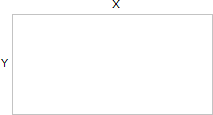
\includegraphics[scale=0.5]{html5_canvas_coordinates.png}
\caption{画布的 X 和 Y 坐标}
\label{html5_canvas_coordinates}
\end{figure}

\subsection{line}


下面的JavaScript代码通过指定从何处开始,在何处结束,来绘制一条线:


\begin{lstlisting}[language=JavaScript]
<script type="text/javascript">
  var c=document.getElementById("drawline");
  var cxt=c.getContext("2d");
  cxt.moveTo(10,10);
  cxt.lineTo(150,50);
  cxt.lineTo(10,50);
  cxt.stroke();
</script>
\end{lstlisting}

相应的canvas 元素:

\begin{lstlisting}[language=HTML]
<canvas id="drawline" width="200" height="100" 
style="border:1px solid #c3c3c3;">
Your browser does not support the canvas element.
</canvas>
\end{lstlisting}




\subsection{circle}


通过规定尺寸、颜色和位置,来绘制一个圆,JavaScript 代码如下:


\begin{lstlisting}[language=JavaScript]
<script type="text/javascript">
  var c=document.getElementById("drawcircle");
  var cxt=c.getContext("2d");
  cxt.fillStyle="#FF0000";
  cxt.beginPath();
  cxt.arc(70,18,15,0,Math.PI*2,true);
  cxt.closePath();
  cxt.fill();
</script>
\end{lstlisting}


相应的canvas 元素:

\begin{lstlisting}[language=HTML]
<canvas id="drawcircle" width="200" height="100" 
style="border:1px solid #c3c3c3;">
Your browser does not support the canvas element.
</canvas>
\end{lstlisting}

\subsection{gradient}


使用指定的颜色来绘制渐变背景,JavaScript 代码如下:

\begin{lstlisting}[language=JavaScript]
<script type="text/javascript">
  var c=document.getElementById("myCanvas");
  var cxt=c.getContext("2d");
  var grd=cxt.createLinearGradient(0,0,175,50);
  grd.addColorStop(0,"#FF0000");
  grd.addColorStop(1,"#00FF00");
  cxt.fillStyle=grd;
  cxt.fillRect(0,0,175,50);
</script>
\end{lstlisting}

相应的canvas 元素:


\begin{lstlisting}[language=HTML]
<canvas id="myCanvas" width="200" height="100" 
style="border:1px solid #c3c3c3;">
Your browser does not support the canvas element.
</canvas>
\end{lstlisting}


\subsection{image}

通过canvas预算,可以把一幅图像放置到画布上,JavaScript代码如下:


\begin{lstlisting}[language=JavaScript]
<script type="text/javascript">
  var c=document.getElementById("myCanvas");
  var cxt=c.getContext("2d");
  var img=new Image()
  img.src="flower.png"
  cxt.drawImage(img,0,0);
</script>
\end{lstlisting}

相应的canvas 元素:

\begin{lstlisting}[language=HTML]
<canvas id="myCanvas" width="200" height="100" 
style="border:1px solid #c3c3c3;">
Your browser does not support the canvas element.
</canvas>
\end{lstlisting}


\begin{longtable}{|p{120pt}|p{270pt}|}
%head
\multicolumn{2}{r}{}
\tabularnewline\hline
属性		&描述
\endhead
%endhead

%firsthead
\caption{HTML5 Canvas 属性}\\
\hline
属性		&描述
\endfirsthead
%endfirsthead

%foot
\multicolumn{2}{r}{}
\endfoot
%endfoot

%lastfoot
\endlastfoot
%endlastfoot

\hline
\multicolumn{2}{|l|}{颜色、样式和阴影}\\
\hline
fillStyle			&设置或返回用于填充绘画的颜色、渐变或模式\\
\hline
strokeStyle		&设置或返回用于笔触的颜色、渐变或模式\\
\hline
shadowColor		&设置或返回用于阴影的颜色\\
\hline
shadowBlur		&设置或返回用于阴影的模糊级别\\
\hline
shadowOffsetX	&设置或返回阴影距形状的水平距离\\
\hline
shadowOffsetY	&设置或返回阴影距形状的垂直距离\\
\hline
\multicolumn{2}{|l|}{线条样式}	\\
\hline
lineCap			&设置或返回线条的结束端点样式\\
\hline
lineJoin			&设置或返回两条线相交时,所创建的拐角类型\\
\hline
lineWidth			&设置或返回当前的线条宽度\\
\hline
miterLimit		&设置或返回最大斜接长度\\
\hline
\multicolumn{2}{|l|}{文本}\\
\hline
font				&设置或返回文本内容的当前字体属性\\
\hline
textAlign			&设置或返回文本内容的当前对齐方式\\
\hline
textBaseline		&设置或返回在绘制文本时使用的当前文本基线\\
\hline
\multicolumn{2}{|l|}{像素操作}\\
\hline
width			&返回 ImageData 对象的宽度\\
\hline
height			&返回 ImageData 对象的高度\\
\hline
data				&返回一个对象,其包含指定的 ImageData 对象的图像数据\\
\hline
\multicolumn{2}{|l|}{合成}\\
\hline
globalAlpha		&设置或返回绘图的当前 alpha 或透明值\\
\hline
globalCompositeOperation&	设置或返回新图像如何绘制到已有的图像上\\
\hline
\end{longtable}


\begin{longtable}{|p{120pt}|p{270pt}|}
%head
\multicolumn{2}{r}{}
\tabularnewline\hline
方法		&描述
\endhead
%endhead

%firsthead
\caption{HTML5 Canvas 方法}\\
\hline
方法		&描述
\endfirsthead
%endfirsthead

%foot
\multicolumn{2}{r}{}
\endfoot
%endfoot

%lastfoot
\endlastfoot
%endlastfoot

\hline
\multicolumn{2}{|l|}{颜色、样式和阴影}\\
\hline
createLinearGradient()	&创建线性渐变(用在画布内容上)\\
\hline
createPattern()		&在指定的方向上重复指定的元素\\
\hline
createRadialGradient()	&创建放射状/环形的渐变(用在画布内容上)\\
\hline
addColorStop()		&规定渐变对象中的颜色和停止位置\\
\hline
\multicolumn{2}{|l|}{矩形}	\\
\hline
rect()				&创建矩形\\
\hline
fillRect()				&绘制“被填充”的矩形\\
\hline
strokeRect()			&绘制矩形(无填充)\\
\hline
clearRect()			&在给定的矩形内清除指定的像素\\
\hline
\multicolumn{2}{|l|}{路径}\\
\hline
fill()					&填充当前绘图(路径)\\
\hline
stroke()				&绘制已定义的路径\\
\hline
beginPath()			&起始一条路径,或重置当前路径\\
\hline
moveTo()				&把路径移动到画布中的指定点,不创建线条\\
\hline
closePath()			&创建从当前点回到起始点的路径\\
\hline
lineTo()				&添加一个新点,然后在画布中创建从该点到最后指定点的线条\\
\hline
clip()				&从原始画布剪切任意形状和尺寸的区域\\
\hline
quadraticCurveTo()		&创建二次贝塞尔曲线\\
\hline
bezierCurveTo()		&创建三次方贝塞尔曲线\\
\hline
arc()					&创建弧/曲线(用于创建圆形或部分圆)\\
\hline
arcTo()				&创建两切线之间的弧/曲线\\
\hline
isPointInPath()		&如果指定的点位于当前路径中,则返回 true,否则返回 false\\
\hline
\multicolumn{2}{|l|}{转换}\\
\hline
scale()				&缩放当前绘图至更大或更小\\
\hline
rotate()				&旋转当前绘图\\
\hline
translate()			&重新映射画布上的 (0,0) 位置\\
\hline
transform()			&替换绘图的当前转换矩阵\\
\hline
setTransform()		&将当前转换重置为单位矩阵。然后运行 transform()\\
\hline
\multicolumn{2}{|l|}{文本}\\
\hline
fillText()				&在画布上绘制“被填充的”文本\\
\hline
strokeText()			&在画布上绘制文本(无填充)\\
\hline
measureText()			&返回包含指定文本宽度的对象\\
\hline
\multicolumn{2}{|l|}{图像绘制}\\
\hline
drawImage()			&向画布上绘制图像、画布或视频\\
\hline
\multicolumn{2}{|l|}{像素操作}\\
\hline
createImageData()		&创建新的、空白的 ImageData 对象\\
\hline
getImageData()		&返回 ImageData 对象,该对象为画布上指定的矩形复制像素数据\\
\hline
putImageData()		&把图像数据(从指定的 ImageData 对象)放回画布上\\
\hline
\multicolumn{2}{|l|}{其他}\\
\hline
save()				&保存当前环境的状态\\
\hline
restore()				&返回之前保存过的路径状态和属性\\
\hline
createEvent()	 		&		\\
\hline
getContext()	 		&		\\
\hline
toDataURL()	 		&		\\
\hline
\end{longtable}

\section{Canvas \& SVG}




HTML5 同时支持内联 SVG和画布,SVG 元素可以直接嵌入 HTML 页面中:

\begin{lstlisting}[language=HTML]
<!DOCTYPE html>
<html>
<body>
<svg xmlns="http://www.w3.org/2000/svg" version="1.1" height="190">
  <polygon points="100,10 40,180 190,60 10,60 160,180"
  style="fill:lime;stroke:purple;stroke-width:5;fill-rule:evenodd;" />
</svg>
</body>
</html>
\end{lstlisting}


SVG相比其他图像格式(比如 JPEG 和 GIF)的优势在于:

\begin{compactitem}
\item SVG 图像可通过文本编辑器来创建和修改
\item SVG 图像可被搜索、索引、脚本化或压缩
\item SVG 是可伸缩的
\item SVG 图像可在任何的分辨率下被高质量地打印
\item SVG 可在图像质量不下降的情况下被放大
\end{compactitem}

Internet Explorer 9、Firefox、Opera、Chrome 以及 Safari 支持内联 SVG。

尽管Canvas 和 SVG 都允许开发者在浏览器中创建图形,但是它们在根本上是不同的。



SVG 是一种使用 XML 描述 2D 图形的语言。在 SVG 中,每个被绘制的图形均被视为对象。如果 SVG 对象的属性发生变化,那么浏览器能够自动重现图形,因此基于 XML的SVG DOM 中的每个元素都是可用的,开发者可以为某个元素附加 JavaScript 事件处理器。

Canvas 通过 JavaScript 来绘制 2D 图形,而且Canvas 是逐像素进行渲染的,因此在<canvas>中,一旦图形被绘制完成,它就不会继续得到浏览器的关注。如果其位置发生变化,那么整个场景也需要重新绘制,包括任何或许已被图形覆盖的对象。


下表列出了 canvas 与 SVG 之间的一些不同之处。

\begin{compactitem}
\item Canvas
	\begin{compactitem}
	\item 依赖分辨率
	\item 不支持事件处理器
	\item 弱的文本渲染能力
	\item 能够以 .png 或 .jpg 格式保存结果图像
	\item 最适合图像密集型的游戏,其中的许多对象会被频繁重绘
	\end{compactitem}
\item SVG
	\begin{compactitem}
	\item 不依赖分辨率
	\item 支持事件处理器
	\item 最适合带有大型渲染区域的应用程序(比如谷歌地图)
	\item 复杂度高会减慢渲染速度(任何过度使用 DOM 的应用都不快)
	\item 不适合游戏应用
	\end{compactitem}
\end{compactitem}




\section{HTML 5 Media}


HTML5 提供了播放音频/视频的标准。

直到现在,仍然不存在一项旨在网页上播放音频/视频的标准。大多数音频/视频是通过插件(比如 Flash、Quicktime等)来播放的。然而,并非所有浏览器都拥有同样的插件。

HTML5 规定了通过audio/video元素来包含音频/视频的标准方法。audio 元素能够播放声音文件或者音频流,video元素用来播放视频文件或者视频流。



\subsection{<audio></audio>}

当前,audio 元素支持三种音频格式:

\begin{compactitem}
\item Ogg Vorbis
\item MP3
\item Wav
\end{compactitem}

要在 HTML5 中播放音频,开发者所有需要的是:

\begin{lstlisting}[language=HTML]
<audio src="song.ogg" controls="controls"></audio>
\end{lstlisting}

其中,control 属性供添加播放、暂停和音量控件。<audio> 与 </audio> 之间插入的内容是供不支持 audio 元素的浏览器显示的:

\begin{lstlisting}[language=HTML]
<audio src="song.ogg" controls="controls">
Your browser does not support the audio tag.
</audio>
\end{lstlisting}

上面的例子使用一个 Ogg 文件,适用于Firefox、Opera 以及 Chrome 浏览器。

要确保适用于 Safari 浏览器,音频文件必须是 MP3 或 Wav 类型。

audio 元素允许多个 source 元素。source 元素可以链接不同的音频文件。浏览器将使用第一个可识别的格式:



\begin{lstlisting}[language=HTML]
<audio controls="controls">
  <source src="song.ogg" type="audio/ogg">
  <source src="song.mp3" type="audio/mpeg">
Your browser does not support the audio tag.
</audio>
\end{lstlisting}

Internet Explorer 8 不支持 audio 元素。在 IE 9 中,将提供对 audio 元素的支持。




\subsection{<video></video>}

当前,video 元素支持三种视频格式:

\begin{compactitem}
\item Ogg
\item MPEG 4
\item WebM
\end{compactitem}

其中:

\begin{compactitem}
\item[*] Ogg = 带有 Theora 视频编码和 Vorbis 音频编码的 Ogg 文件
\item[*] MPEG4 = 带有 H.264 视频编码和 AAC 音频编码的 MPEG 4 文件
\item[*] WebM = 带有 VP8 视频编码和 Vorbis 音频编码的 WebM 文件
\end{compactitem}


要在 HTML5 中显示视频,最简单的代码是:

\begin{lstlisting}[language=HTML]
<video src="movie.ogg" controls="controls"></video>
\end{lstlisting}

其中,control 属性供添加播放、暂停和音量控件,而且包含宽度和高度属性也是不错的主意。


<video> 与 </video> 之间插入的内容是供不支持 video 元素的浏览器显示的:

\begin{lstlisting}[language=HTML]
<video src="movie.ogg" width="320" height="240" controls="controls">
Your browser does not support the video tag.
</video>
\end{lstlisting}

上面的例子使用一个 Ogg 文件,适用于Firefox、Opera 以及 Chrome 浏览器。若要适用于 Safari 浏览器,视频文件必须是 MPEG4 类型。

video 元素允许多个 source 元素。source 元素可以链接不同的视频文件,浏览器将使用第一个可识别的格式:

\begin{lstlisting}[language=HTML]
<video width="320" height="240" controls="controls">
  <source src="movie.ogg" type="video/ogg">
  <source src="movie.mp4" type="video/mp4">
Your browser does not support the video tag.
</video>
\end{lstlisting}


Internet Explorer 8 不支持 video 元素。在 IE 9 中,将提供对使用 MPEG4 的 video 元素的支持。






HTML5 <video> 元素同样拥有方法、属性和事件。其中,方法用于播放、暂停以及加载等,属性(比如时长、音量等)可以被读取或设置,而DOM事件能够通知用户,比方说,<video> 元素开始播放、已暂停,已停止,等等。

下例中简单的方法演示了如何使用 <video> 元素,读取并设置属性,以及如何调用方法。

\begin{lstlisting}[language=HTML]
<div style="text-align:center;">
  <button onclick="playPause()">播放/暂停</button> 
  <button onclick="makeBig()">大</button>
  <button onclick="makeNormal()">中</button>
  <button onclick="makeSmall()">小</button>
  <br /> 
  <video id="video1" width="420" style="margin-top:15px;">
    <source src="/example/html5/mov_bbb.mp4" type="video/mp4" />
    <source src="/example/html5/mov_bbb.ogg" type="video/ogg" />
    Your browser does not support HTML5 video.
  </video>
</div> 

<script type="text/javascript">
  var myVideo=document.getElementById("video1");
  function playPause()
  { 
  if (myVideo.paused) 
    myVideo.play(); 
  else 
   myVideo.pause(); 
  } 

  function makeBig()
  { 
    myVideo.width=560; 
  } 

  function makeSmall()
  { 
    myVideo.width=320; 
  } 

  function makeNormal()
  { 
    myVideo.width=420; 
  } 
</script> 
\end{lstlisting}

上面的例子调用了两个方法:play() 和 pause(),它同时使用了两个属性:paused 和 width。


HTML5 DOM 为 <audio> 和 <video> 元素提供了方法、属性和事件。这些方法、属性和事件允许开发者使用 JavaScript 来操作 <audio> 和 <video> 元素。



\begin{longtable}{|p{80pt}|p{280pt}|}
%head
\multicolumn{2}{r}{}
\tabularnewline\hline
方法		&描述
\endhead
%endhead

%firsthead
\caption{HTML5 Audio/Video 方法}\\
\hline
方法		&描述
\endfirsthead
%endfirsthead

%foot
\multicolumn{2}{r}{}
\endfoot
%endfoot

%lastfoot
\endlastfoot
%endlastfoot

\hline
addTextTrack()	&向音频/视频添加新的文本轨道\\
\hline
canPlayType()		&检测浏览器是否能播放指定的音频/视频类型\\
\hline
load()			&重新加载音频/视频元素\\
\hline
play()			&开始播放音频/视频\\
\hline
pause()			&暂停当前播放的音频/视频\\
\hline
\end{longtable}


\begin{longtable}{|p{80pt}|p{280pt}|}
%head
\multicolumn{2}{r}{}
\tabularnewline\hline
属性		&描述
\endhead
%endhead

%firsthead
\caption{HTML5 Audio/Video 属性}\\
\hline
属性		&描述
\endfirsthead
%endfirsthead

%foot
\multicolumn{2}{r}{}
\endfoot
%endfoot

%lastfoot
\endlastfoot
%endlastfoot

\hline
audioTracks		&返回表示可用音轨的 AudioTrackList 对象\\
\hline
autoplay			&设置或返回是否在加载完成后随即播放音频/视频\\
\hline
buffered			&返回表示音频/视频已缓冲部分的 TimeRanges 对象\\
\hline
controller		&返回表示音频/视频当前媒体控制器的 MediaController 对象\\
\hline
controls			&设置或返回音频/视频是否显示控件(比如播放/暂停等)\\
\hline
crossOrigin		&设置或返回音频/视频的 CORS 设置\\
\hline
currentSrc		&返回当前音频/视频的 URL\\
\hline
currentTime		&设置或返回音频/视频中的当前播放位置(以秒计)\\
\hline
defaultMuted		&设置或返回音频/视频默认是否静音\\
\hline
defaultPlaybackRate&设置或返回音频/视频的默认播放速度\\
\hline
duration			&返回当前音频/视频的长度(以秒计)\\
\hline
ended			&返回音频/视频的播放是否已结束\\
\hline
error			&返回表示音频/视频错误状态的 MediaError 对象\\
\hline
loop				&设置或返回音频/视频是否应在结束时重新播放\\
\hline
mediaGroup		&设置或返回音频/视频所属的组合(用于连接多个音频/视频元素)\\
\hline
muted			&设置或返回音频/视频是否静音\\
\hline
networkState		&返回音频/视频的当前网络状态\\
\hline
paused			&设置或返回音频/视频是否暂停\\
\hline
playbackRate		&设置或返回音频/视频播放的速度\\
\hline
played			&返回表示音频/视频已播放部分的 TimeRanges 对象\\
\hline
preload			&设置或返回音频/视频是否应该在页面加载后进行加载 \newline 如果使用``autoplay",则忽略该属性。\\
\hline
readyState		&返回音频/视频当前的就绪状态\\
\hline
seekable			&返回表示音频/视频可寻址部分的 TimeRanges 对象\\
\hline
seeking			&返回用户是否正在音频/视频中进行查找\\
\hline
src				&设置或返回音频/视频元素的当前来源\\
\hline
startDate			&返回表示当前时间偏移的 Date 对象\\
\hline
textTracks		&返回表示可用文本轨道的 TextTrackList 对象\\
\hline
videoTracks		&返回表示可用视频轨道的 VideoTrackList 对象\\
\hline
volume			&设置或返回音频/视频的音量\\
\hline
\end{longtable}




\begin{longtable}{|p{80pt}|p{280pt}|}
%head
\multicolumn{2}{r}{}
\tabularnewline\hline
事件		&描述
\endhead
%endhead

%firsthead
\caption{HTML5 Audio/Video 事件}\\
\hline
事件		&描述
\endfirsthead
%endfirsthead

%foot
\multicolumn{2}{r}{}
\endfoot
%endfoot

%lastfoot
\endlastfoot
%endlastfoot

\hline
abort			&当音频/视频的加载已放弃时\\
\hline
canplay			&当浏览器可以播放音频/视频时\\
\hline
canplaythrough	&当浏览器可在不因缓冲而停顿的情况下进行播放时\\
\hline
durationchange	&当音频/视频的时长已更改时\\
\hline
emptied			&当目前的播放列表为空时\\
\hline
ended			&当目前的播放列表已结束时\\
\hline
error			&当在音频/视频加载期间发生错误时\\
\hline
loadeddata		&当浏览器已加载音频/视频的当前帧时\\
\hline
loadedmetadata	&当浏览器已加载音频/视频的元数据时\\
\hline
loadstart			&当浏览器开始查找音频/视频时\\
\hline
pause			&当音频/视频已暂停时\\
\hline
play				&当音频/视频已开始或不再暂停时\\
\hline
playing			&当音频/视频在已因缓冲而暂停或停止后已就绪时\\
\hline
progress			&当浏览器正在下载音频/视频时\\
\hline
ratechange		&当音频/视频的播放速度已更改时\\
\hline
seeked			&当用户已移动/跳跃到音频/视频中的新位置时\\
\hline
seeking			&当用户开始移动/跳跃到音频/视频中的新位置时\\
\hline
stalled			&当浏览器尝试获取媒体数据,但数据不可用时\\
\hline
suspend			&当浏览器刻意不获取媒体数据时\\
\hline
timeupdate		&当目前的播放位置已更改时\\
\hline
volumechange		&当音量已更改时\\
\hline
waiting			&当视频由于需要缓冲下一帧而停止\\
\hline
\end{longtable}


注释:在所有属性中,只有 videoWidth 和 videoHeight 属性是立即可用的。在视频的元数据已加载后,其他属性才可用。







\section{Cache Manifest}

HTML5 引入了应用程序缓存(Application Cache)\footnote{所有主流浏览器均支持应用程序缓存,除了 Internet Explorer。},这意味着 web 应用可进行缓存,并可在没有因特网连接时进行访问。使用 HTML5,通过创建 cache manifest 文件,从而可以轻松地创建 web 应用的离线版本。

应用程序缓存为应用带来三个优势:

\begin{compactitem}
\item 离线浏览 - 用户可在应用离线时使用它们
\item 速度 - 已缓存资源加载得更快
\item 减少服务器负载 - 浏览器将只从服务器下载更新过或更改过的资源。
\end{compactitem}

要启用应用程序缓存,需要在文档的 <html> 标签中包含 manifest 属性,下面的示例展示了带有 cache manifest 的 HTML 文档(供离线浏览):

\begin{lstlisting}[language=HTML]
<!DOCTYPE HTML>
<html manifest="demo.appcache">
<body>
The content of the document......
</body>
</html>
\end{lstlisting}

每个指定了 manifest 的页面在用户对其访问时都会被缓存。如果未指定 manifest 属性,则页面不会被缓存(除非在 manifest 文件\footnote{manifest 文件的建议的文件扩展名是:".appcache"。}中直接指定了该页面)。

manifest 文件是简单的文本文件,它告知浏览器被缓存的内容(以及不缓存的内容),manifest 文件可分为三个部分:

\begin{compactitem}
\item CACHE MANIFEST - 在此标题下列出的文件将在首次下载后进行缓存
\item NETWORK - 在此标题下列出的文件需要与服务器的连接,且不会被缓存
\item FALLBACK - 在此标题下列出的文件规定当页面无法访问时的回退页面(比如 404 页面)
\end{compactitem}



manifest 文件需要配置正确的 MIME-type,即 "text/cache-manifest",而且必须在 web 服务器上进行配置。


一个完整的 Manifest 文件\footnote{注释:以 "\#" 开头的是注释行,但也可满足其他用途。应用的缓存会在其 manifest 文件更改时被更新。如果您编辑了一幅图片,或者修改了一个 JavaScript 函数,这些改变都不会被重新缓存。更新注释行中的日期和版本号是一种使浏览器重新缓存文件的办法。}如下:

\begin{lstlisting}[language=bash]
CACHE MANIFEST
# 2012-02-21 v1.0.0
/theme.css
/logo.gif
/main.js

NETWORK:
login.asp

FALLBACK:
/html5/ /404.html
\end{lstlisting}

其中:



\begin{compactenum}
\item CACHE MANIFEST

第一行,CACHE MANIFEST,是必需的:

\begin{lstlisting}[language=bash]
CACHE MANIFEST
/theme.css
/logo.gif
/main.js
\end{lstlisting}

上面的 manifest 文件列出了三个资源:一个 CSS 文件,一个 GIF 图像,以及一个 JavaScript 文件。当 manifest 文件加载后,浏览器会从网站的根目录下载这三个文件。然后,无论用户何时与因特网断开连接,这些资源依然是可用的。



\item NETWORK

下面的 NETWORK 小节规定文件 "login.asp" 永远不会被缓存,且离线时是不可用的:

\begin{lstlisting}[language=bash]
NETWORK:
login.asp
\end{lstlisting}

可以使用星号来指示所有其他其他资源/文件都需要因特网连接:

\begin{lstlisting}[language=bash]
NETWORK:
*
\end{lstlisting}



\item FALLBACK

下面的 FALLBACK 小节规定如果无法建立因特网连接,则用``offline.html"\footnote{第一个 URI 是资源,第二个是替补。} 替代 /html5/ 目录中的所有文件:

\begin{lstlisting}[language=bash]
FALLBACK:
/html5/ /404.html
\end{lstlisting}



\end{compactenum}



一旦应用被缓存,则浏览器会继续展示已缓存的版本,即使后来修改了服务器上的文件,浏览器会保持缓存直到发生下列情况:

\begin{compactitem}
\item 用户清空浏览器缓存
\item manifest 文件被修改\footnote{一旦文件被缓存,则浏览器会继续展示已缓存的版本,即使修改了服务器上的文件。为了确保浏览器更新缓存,需要更新 manifest 文件。}
\item 由程序来更新应用缓存
\end{compactitem}

另外,浏览器对缓存数据的容量限制可能不太一样(某些浏览器设置的限制是每个站点 5MB)。



\section{Drag and drop}




拖放\footnote{Internet Explorer 9、Firefox、Opera 12、Chrome 以及 Safari 5 支持拖放,但是在 Safari 5.1.2 中不支持拖放。}(Drag 和 drop)是一种常见的特性,即抓取对象以后拖到另一个位置,现在拖放是 HTML5 标准的组成部分,任何元素都能够拖放。

下面的例子是一个简单的拖放实例:


\begin{lstlisting}[language=HTML]
<!DOCTYPE HTML>
<html>
<head>
<script type="text/javascript">
function allowDrop(ev)
{
ev.preventDefault();
}

function drag(ev)
{
ev.dataTransfer.setData("Text",ev.target.id);
}

function drop(ev)
{
ev.preventDefault();
var data=ev.dataTransfer.getData("Text");
ev.target.appendChild(document.getElementById(data));
}
</script>
</head>
<body>

<div id="div1" ondrop="drop(event)"
ondragover="allowDrop(event)"></div>
<img id="drag1" src="img_logo.gif" draggable="true"
ondragstart="drag(event)" width="336" height="69" />

</body>
</html>
\end{lstlisting}

\begin{compactenum}
\item draggable



首先,为了使元素可拖动,把 draggable 属性设置为 true :

\begin{lstlisting}[language=HTML]
<img draggable="true" />
\end{lstlisting}


\item ondragstart 和 setData()


然后,ondragstart 和 setData()规定当元素被拖动时,会发生什么。在上面的例子中,ondragstart 属性调用了一个函数,drag(event),它规定了被拖动的数据。

dataTransfer.setData() 方法设置被拖数据的数据类型和值:



\begin{lstlisting}[language=JavaScript]
function drag(ev)
{
  ev.dataTransfer.setData("Text",ev.target.id);
}
\end{lstlisting}


在这个例子中,数据类型是 "Text",值是可拖动元素的 id ("drag1")。

默认地,无法将数据/元素放置到其他元素中。如果需要设置允许放置,我们必须阻止对元素的默认处理方式,使用ondragover 事件规定在何处放置被拖动的数据。

\item ondragover

下面通过调用 ondragover 事件的 event.preventDefault() 方法来设置允许放置:


\begin{lstlisting}[language=JavaScript]
event.preventDefault()
\end{lstlisting}

\item ondrop

当放置被拖数据时,会发生 ondrop 事件。在上面的例子中,ondrop 属性调用了一个函数,drop(event):

\begin{lstlisting}[language=JavaScript]
function drop(ev)
{
  ev.preventDefault();
  var data=ev.dataTransfer.getData("Text");
  ev.target.appendChild(document.getElementById(data));
}
\end{lstlisting}


\end{compactenum}

最后,代码解释:

\begin{compactitem}
\item 调用 preventDefault() 来避免浏览器对数据的默认处理(drop 事件的默认行为是以链接形式打开)
\item 通过 dataTransfer.getData("Text") 方法获得被拖的数据。该方法将返回在 setData() 方法中设置为相同类型的任何数据。
\item 被拖数据是被拖元素的 id ("drag1")
\item 把被拖元素追加到放置元素(目标元素)中
\end{compactitem}







\section{Web storage}




	






HTML5 提供了两种在客户端存储数据的新方法:

\begin{compactitem}
\item localStorage - 没有时间限制的数据存储
\item sessionStorage - 针对一个 session 的数据存储
\end{compactitem}


之前,这些都是由 cookie 完成的。但是 cookie 不适合大量数据的存储,因为它们由每个对服务器的请求来传递,这使得 cookie 速度很慢而且效率也不高。

在 HTML5 中,HTML5 使用 JavaScript 来存储和访问数据,而且数据不是由每个服务器请求传递的,而是只有在请求时使用数据,这样就使得在不影响网站性能的情况下存储大量数据成为可能。

对于不同的网站,数据存储于不同的区域,并且一个网站只能访问其自身的数据。

\subsection{localStorage 方法}

localStorage 方法存储的数据没有时间限制。第二天、第二周或下一年之后,数据依然可用。

下面是创建和访问 localStorage的示例:



\begin{lstlisting}[language=JavaScript]
<script type="text/javascript">
localStorage.lastname="Smith";
document.write(localStorage.lastname);
</script>
\end{lstlisting}

下面的例子对用户访问页面的次数进行计数:


\begin{lstlisting}[language=JavaScript]
<script type="text/javascript">
  if (localStorage.pagecount)
  {
    localStorage.pagecount=Number(localStorage.pagecount) +1;
  }
  else
  {
    localStorage.pagecount=1;
  }
document.write("Visits "+ localStorage.pagecount + " time(s).");
</script>
\end{lstlisting}



\subsection{sessionStorage 方法}

sessionStorage 方法针对一个 session 进行数据存储。当用户关闭浏览器窗口后,数据会被删除。


下面创建并访问一个 sessionStorage的示例:

\begin{lstlisting}[language=JavaScript]
<script type="text/javascript">
sessionStorage.lastname="Smith";
document.write(sessionStorage.lastname);
</script>
\end{lstlisting}

下面的例子对用户在当前 session 中访问页面的次数进行计数:

\begin{lstlisting}[language=JavaScript]
<script type="text/javascript">
  if (sessionStorage.pagecount)
  {
  sessionStorage.pagecount=Number(sessionStorage.pagecount) +1;
  }
  else
  {
  sessionStorage.pagecount=1;
  }
document.write("Visits "+sessionStorage.pagecount+" time(s) this session.");
</script>
\end{lstlisting}




\section{Geolocation}


HTML5 Geolocation(地理定位)API用于定位用户的地理位置\footnote{鉴于该特性可能侵犯用户的隐私,除非用户同意,否则用户位置信息是不可用的。}。


Internet Explorer 9、Firefox、Chrome、Safari 以及 Opera 支持地理定位,而且对于拥有 GPS 的设备,比如 iPhone,地理定位更加精确。

在HTML5应用中,可以使用 getCurrentPosition() 方法来获得用户的位置,下面是一个简单的地理定位实例,可返回用户位置的经度和纬度。

\begin{lstlisting}[language=JavaScript]
<script>
var x=document.getElementById("demo");
function getLocation()
  {
  if (navigator.geolocation)
    {
    navigator.geolocation.getCurrentPosition(showPosition);
    }
  else{x.innerHTML="Geolocation is not supported by this browser.";}
  }
function showPosition(position)
  {
  x.innerHTML="Latitude: " + position.coords.latitude +
  "<br />Longitude: " + position.coords.longitude;
  }
</script>
\end{lstlisting}


这里展示的过程包括:

\begin{compactenum}
\item 检测是否支持地理定位
\item 如果支持,则运行 getCurrentPosition() 方法。如果不支持,则向用户显示一段消息。
\item 如果getCurrentPosition()运行成功,则向参数showPosition中规定的函数返回一个coordinates对象
\item showPosition() 函数获得并显示经度和纬度
\end{compactenum}




这个例子是一个非常基础的地理定位脚本,不含错误处理。getCurrentPosition() 方法的第二个参数用于处理错误。它规定当获取用户位置失败时运行的函数:


\begin{lstlisting}[language=JavaScript]
function showError(error)
  {
  switch(error.code)
    {
    case error.PERMISSION_DENIED:
      x.innerHTML="User denied the request for Geolocation."
      break;
    case error.POSITION_UNAVAILABLE:
      x.innerHTML="Location information is unavailable."
      break;
    case error.TIMEOUT:
      x.innerHTML="The request to get user location timed out."
      break;
    case error.UNKNOWN_ERROR:
      x.innerHTML="An unknown error occurred."
      break;
    }
  }
\end{lstlisting}

其中可能会使用到的错误处理代码的意义分别是:

\begin{compactenum}
\item Permission denied - 用户不允许地理定位
\item Position unavailable - 无法获取当前位置
\item Timeout - 操作超时
\end{compactenum}

如需在地图中显示结果,就需要访问可使用经纬度的地图服务,比如谷歌地图:

\begin{lstlisting}[language=JavaScript]
function showPosition(position)
{
var latlon=position.coords.latitude+","+position.coords.longitude;

var img_url="http://maps.googleapis.com/maps/api/staticmap?center="
+latlon+"&zoom=14&size=400x300&sensor=false";

document.getElementById("mapholder").innerHTML="<img src='"+img_url+"' />";
}
\end{lstlisting}

在上例中,使用返回的经纬度数据在谷歌地图中显示位置(使用静态图像)。

另外,地理定位对于给定位置的信息同样很有用处,一些应用场景包括:

\begin{compactitem}
\item 更新本地信息
\item 显示用户周围的兴趣点
\item 交互式车载导航系统 (GPS)
\end{compactitem}

若成功,则 getCurrentPosition() 方法返回对象。始终会返回 latitude、longitude 以及 accuracy 属性。如果可用,则会返回其他下面的属性。


\begin{longtable}{|p{120pt}|p{120pt}|}
%head
\multicolumn{2}{r}{}
\tabularnewline\hline
属性		& 描述
\endhead
%endhead

%firsthead
\caption{HTML 5 <audio>属性}\\
\hline
属性		& 描述
\endfirsthead
%endfirsthead

%foot
\multicolumn{2}{r}{}
\endfoot
%endfoot

%lastfoot
\endlastfoot
%endlastfoot

\hline
coords.latitude	&十进制数的纬度\\
\hline
coords.longitude	&十进制数的经度\\
\hline
coords.accuracy	&位置精度\\
\hline
coords.altitude	&海拔,海平面以上以米计\\
\hline
coords.altitudeAccuracy	&位置的海拔精度\\
\hline
coords.heading	&方向,从正北开始以度计\\
\hline
coords.speed		&速度,以米/每秒计\\
\hline
timestamp		&响应的日期/时间\\
\hline

\end{longtable}


Geolocation 对象的watchPosition()方法返回用户的当前位置,并继续返回用户移动时的更新位置(就像汽车上的 GPS)。

下面的例子展示 watchPosition() 方法,这里需要一台精确的 GPS 设备来测试该示例(比如 iPhone):

\begin{lstlisting}[language=JavaScript]
<script>
var x=document.getElementById("demo");
function getLocation()
  {
  if (navigator.geolocation)
    {
    navigator.geolocation.watchPosition(showPosition);
    }
  else{x.innerHTML="Geolocation is not supported by this browser.";}
  }
function showPosition(position)
  {
  x.innerHTML="Latitude: " + position.coords.latitude +
  "<br />Longitude: " + position.coords.longitude;
  }
</script>
\end{lstlisting}

最后,使用clearWatch()方法停止 watchPosition(),结束。


\section{Web Workers}

当在 HTML 页面中执行脚本时,页面的状态是不可响应的,直到脚本已完成。

web worker 是运行在后台的 JavaScript,独立于其他脚本,不会影响页面的性能。开发者可以继续做任何愿意做的事情:点击、选取内容等等,而此时 web worker 在后台运行。


\begin{compactenum}
\item 检测 Web Worker 支持



除了 Internet Explorer之外,所有主流浏览器均支持 web worker,因此在创建 web worker 之前,需要先检测用户的浏览器是否支持它:

\begin{lstlisting}[language=JavaScript]
  if(typeof(Worker)!=="undefined")
  {
  // Yes! Web worker support!
  // Some code.....
  }
  else
  {
  // Sorry! No Web Worker support..
  }
\end{lstlisting}

\item 创建 web worker 文件

然后,可以在外部 JavaScript 中开始创建我们的 web worker。

在这里,为了实现在后台计数的功能,创建了计数脚本\footnote{注释:web worker 通常不用于如此简单的脚本,而是用于更耗费 CPU 资源的任务。}。该脚本存储于 "demo\_workers.js" 文件中:

\begin{lstlisting}[language=JavaScript]
var i=0;

function timedCount()
{
i=i+1;
postMessage(i);
setTimeout("timedCount()",500);
}

timedCount();
\end{lstlisting}

以上代码中重要的部分是 postMessage() 方法 - 它用于向 HTML 页面传回一段消息。

\item 创建 Web Worker 对象

在具备了 web worker 文件之后,现在就可以从 HTML 页面调用它。下面的代码检测是否存在 worker,如果不存在,- 它会创建一个新的 web worker 对象,然后运行 "demo\_workers.js" 中的代码:

\begin{lstlisting}[language=JavaScript]
  if(typeof(w)=="undefined")
  {
  w=new Worker("demo_workers.js");
  }
\end{lstlisting}

然后我们就可以从 web worker 发生和接收消息了,于是接着向 web worker 添加一个 "onmessage" 事件监听器:

\begin{lstlisting}[language=JavaScript]
w.onmessage=function(event){
  document.getElementById("result").innerHTML=event.data;
};
\end{lstlisting}

当 web worker 传递消息时,会执行事件监听器中的代码。event.data 中存有来自 event.data 的数据。

\item 终止 Web Worker

创建 web worker 对象后,它就会持续监听消息(即使在外部脚本完成之后)直到其被终止为止。

如需终止 web worker,并释放浏览器/计算机资源,可使用 terminate() 方法:

\begin{lstlisting}[language=JavaScript]
w.terminate();
\end{lstlisting}


\end{compactenum}

下面是完整的 Web Worker示例中HTML页面的代码:

\begin{lstlisting}[language=JavaScript]
<!DOCTYPE html>
<html>
<body>
<p>Count numbers: <output id="result"></output></p>
<button onclick="startWorker()">Start Worker</button>
<button onclick="stopWorker()">Stop Worker</button>
<br />
<script>
var w;

function startWorker(){
  if(typeof(Worker)!=="undefined"){
    if(typeof(w)=="undefined"){
      w=new Worker("demo_workers.js");
    }
    w.onmessage = function (event){
      document.getElementById("result").innerHTML=event.data;
    };
  }
  else{
    document.getElementById("result").innerHTML="Sorry, your browser
     does not support Web Workers...";
  }
}

function stopWorker(){
  w.terminate();
}
</script>
</body>
</html>
\end{lstlisting}

由于 web worker 位于外部文件中,它们无法访问下列JavaScript 对象:


\begin{compactitem}
\item window 对象
\item document 对象
\item parent 对象
\end{compactitem}


\section{Server-sent Event}

HTML5 服务器发送事件(server-sent event)允许网页获得来自服务器的更新。

Server-Sent 事件指的是网页自动获取来自服务器的更新(注意是单向消息传递),其实以前也可能做到这一点,前提是网页不得不询问是否有可用的更新。

通过服务器发送事件,更新能够自动到达的例子有:Facebook/Twitter 更新、估价更新、新的博文、赛事结果等。

\begin{compactenum}
\item 检测 Server-Sent 事件支持



所有主流浏览器均支持服务器发送事件,除了 Internet Explorer,因此额外的代码来检测服务器发送事件的浏览器支持情况:

\begin{lstlisting}[language=JavaScript]
  if(typeof(EventSource)!=="undefined") {
  // Yes! Server-sent events support!
  // Some code.....
  }
  else {
  // Sorry! No server-sent events support..
  }
\end{lstlisting}


\item 接收 Server-Sent 事件通知

EventSource 对象用于接收服务器发送事件通知:

\begin{lstlisting}[language=JavaScript]
var source=new EventSource("demo_sse.php");
source.onmessage=function(event) {
    document.getElementById("result").innerHTML+=event.data + "<br />";
  };
\end{lstlisting}

接收服务器发送事件通知的过程如下

\begin{compactitem}
\item 创建一个新的 EventSource 对象,然后规定发送更新的页面的 URL(本例中是 "demo\_sse.php")
\item 每接收到一次更新,就会发生 onmessage 事件
\item 当 onmessage 事件发生时,把已接收的数据推入 id 为 "result" 的元素中
\end{compactitem}




\end{compactenum}


为了让上面的例子可以运行,还需要能够发送数据更新的服务器(比如 PHP 和 ASP)。

服务器端事件流的语法是非常简单,把 "Content-Type" 报头设置为``text/event-stream"就可以开始发送事件流了。

下面分别是实现发送事件流的PHP代码和ASP代码:

PHP 代码 (demo\_sse.php):

\begin{lstlisting}[language=PHP]
<?php
  header('Content-Type: text/event-stream');
  header('Cache-Control: no-cache');

  $time = date('r');
  echo "data: The server time is: {$time}\n\n";
  flush();
?>
\end{lstlisting}


ASP 代码 (VB) (demo\_sse.asp):

\begin{lstlisting}[language=VBScript]
<%
  Response.ContentType="text/event-stream"
  Response.Expires=-1
  Response.Write("data: " & now())
  Response.Flush()
%>
\end{lstlisting}


代码解释:

\begin{compactitem}
\item 把报头 "Content-Type" 设置为 "text/event-stream"
\item 规定不对页面进行缓存
\item 输出发送日期(始终以 "data: " 开头)
\item 向网页刷新输出数据
\end{compactitem}

在上面的例子中,我们使用 onmessage 事件来获取消息。不过还可以使用其他事件。

\begin{longtable}{|p{120pt}|p{120pt}|}
%head
\multicolumn{2}{r}{}
\tabularnewline\hline
事件		& 描述
\endhead
%endhead

%firsthead
\caption{HTML 5 EventSource 对象}\\
\hline
事件		& 描述
\endfirsthead
%endfirsthead

%foot
\multicolumn{2}{r}{}
\endfoot
%endfoot

%lastfoot
\endlastfoot
%endlastfoot
\hline
onopen		&当通往服务器的连接被打开\\
\hline
onmessage	&当接收到消息\\
\hline
onerror		&当错误发生\\
\hline
\end{longtable}



\section{XHTML5}


XHTML5 is the XML serialization of HTML5. XML documents must be served with an XML Internet media type (often confused with MIME type) such as application/xhtml+xml or application/xml. XHTML5 requires XML's strict, well-formed syntax. The choice between HTML5 and XHTML5 boils down to the choice of a MIME/content type: the media type one chooses determines what type of document should be used. In XHTML5, the HTML5 doctype html is optional and may simply be omitted. HTML that has been written to conform to both the HTML and XHTML specifications—and which will therefore produce the same DOM tree whether parsed as HTML or XML—is termed "polyglot markup".



\section{Error handling}

HTML5 is designed so that old browsers can safely ignore new HTML5 constructs.[citation needed] In contrast to HTML 4.01, the HTML5 specification gives detailed rules for lexing and parsing, with the intent that different compliant browsers will produce the same result in the case of incorrect syntax. Although HTML5 now defines a consistent behavior for "tag soup" documents, those documents are not regarded as conforming to the HTML5 standard.


\section{Popularity}

According to a report released on 30 September 2011, 34 of the world's top 100 Web sites were using HTML5 – the adoption led by search engines and social networks. Another report released in July 2013 has shown that 153 of the Fortune 500 U.S. companies already implemented HTML5 on their corporate websites.



\section{Difference from HTML 4.01 and XHTML 1.x}


The following is a cursory list of differences and some specific examples.

\begin{compactitem}
\item New parsing rules: oriented towards flexible parsing and compatibility; not based on SGML
\item Ability to use inline SVG and MathML in text/html
\item New elements: article, aside, audio, bdi, canvas, command, data, datalist, details, embed, figcaption, figure, footer, header, keygen, mark, meter, nav, output, progress, rp, rt, ruby, section, source, summary, time, track, video, wbr
\item New types of form controls: dates and times, email, url, search, number, range, tel, color
\item New attributes: charset (on meta), async (on script)
\item Global attributes (that can be applied for every element): id, tabindex, hidden, data-* (custom data attributes)
\item Deprecated elements will be dropped altogether: acronym, applet, basefont, big, center, dir, font, frame, frameset, isindex, noframes, strike, tt
\end{compactitem}

dev.w3.org provides the latest Editors Draft of "HTML5 differences from HTML 4", which provides a complete outline of additions, removals and changes between HTML5 and HTML 4.



\chapter{Digital Rights Manage}


Industrial players including the BBC, Google, Microsoft, and Netflix have been lobbying for the inclusion of Encrypted Media Extensions (EME), a form of Digital Rights Management (DRM), into the HTML5 standard. As of the end of 2012 and the beginning of 2013, 27 organisations including the Free Software Foundation have started a campaign against including Digital Rights Management in the HTML5 standard. However in late September 2013, the W3C HTML working group decided that Encrypted Media Extensions, a form of DRM was "in scope" and will potentially be included in the HTML 5.1 standard






\chapter{Reconstruction use HTML5}












































